\documentclass[a4paper,10pt]{article}
\usepackage[utf8]{inputenc}
\DeclareMathAlphabet\mathbfcal{OMS}{cmsy}{b}{n}

\usepackage{amsmath,amsfonts,mathrsfs,color,colordvi}
\usepackage{graphicx}
\usepackage{float}

% To get graphics from directory ./images
\graphicspath{{./images/}}

\textwidth 16cm
\textheight 23cm
\topmargin -1.cm
\oddsidemargin 0cm
\evensidemargin 0cm
% \pagestyle{empty}
\begin{document}

\renewcommand{\baselinestretch}{1.25}
 
\title{Preparing a MSWindows installer of DAMQT with Inno Setup}
\author{
Rafael L\'opez\footnote{Universidad Aut\'onoma de
Madrid,
Facultad de Ciencias. Departamento de Qu\'{i}mica F\'{i}sica Aplicada.}{ }}

\maketitle

\large

\section{Preparing software}

The following software must be installed on a machine with MSWindows\copyright:

\begin{enumerate}
\item Qt library including tools. In particular, including Qt creator and mingw32 features.
 
\item Mingw32\copyright{ } and MSYS\copyright.

\item Inno Setup\copyright.

\item Cmake\copyright.

\item DAMQT package.
\end{enumerate}

Figure \ref{fig:1} Shows a typical installation of Qt and MinGW.

\begin{minipage}{0.5\linewidth}
\begin{figure}[H]
\begin{center}
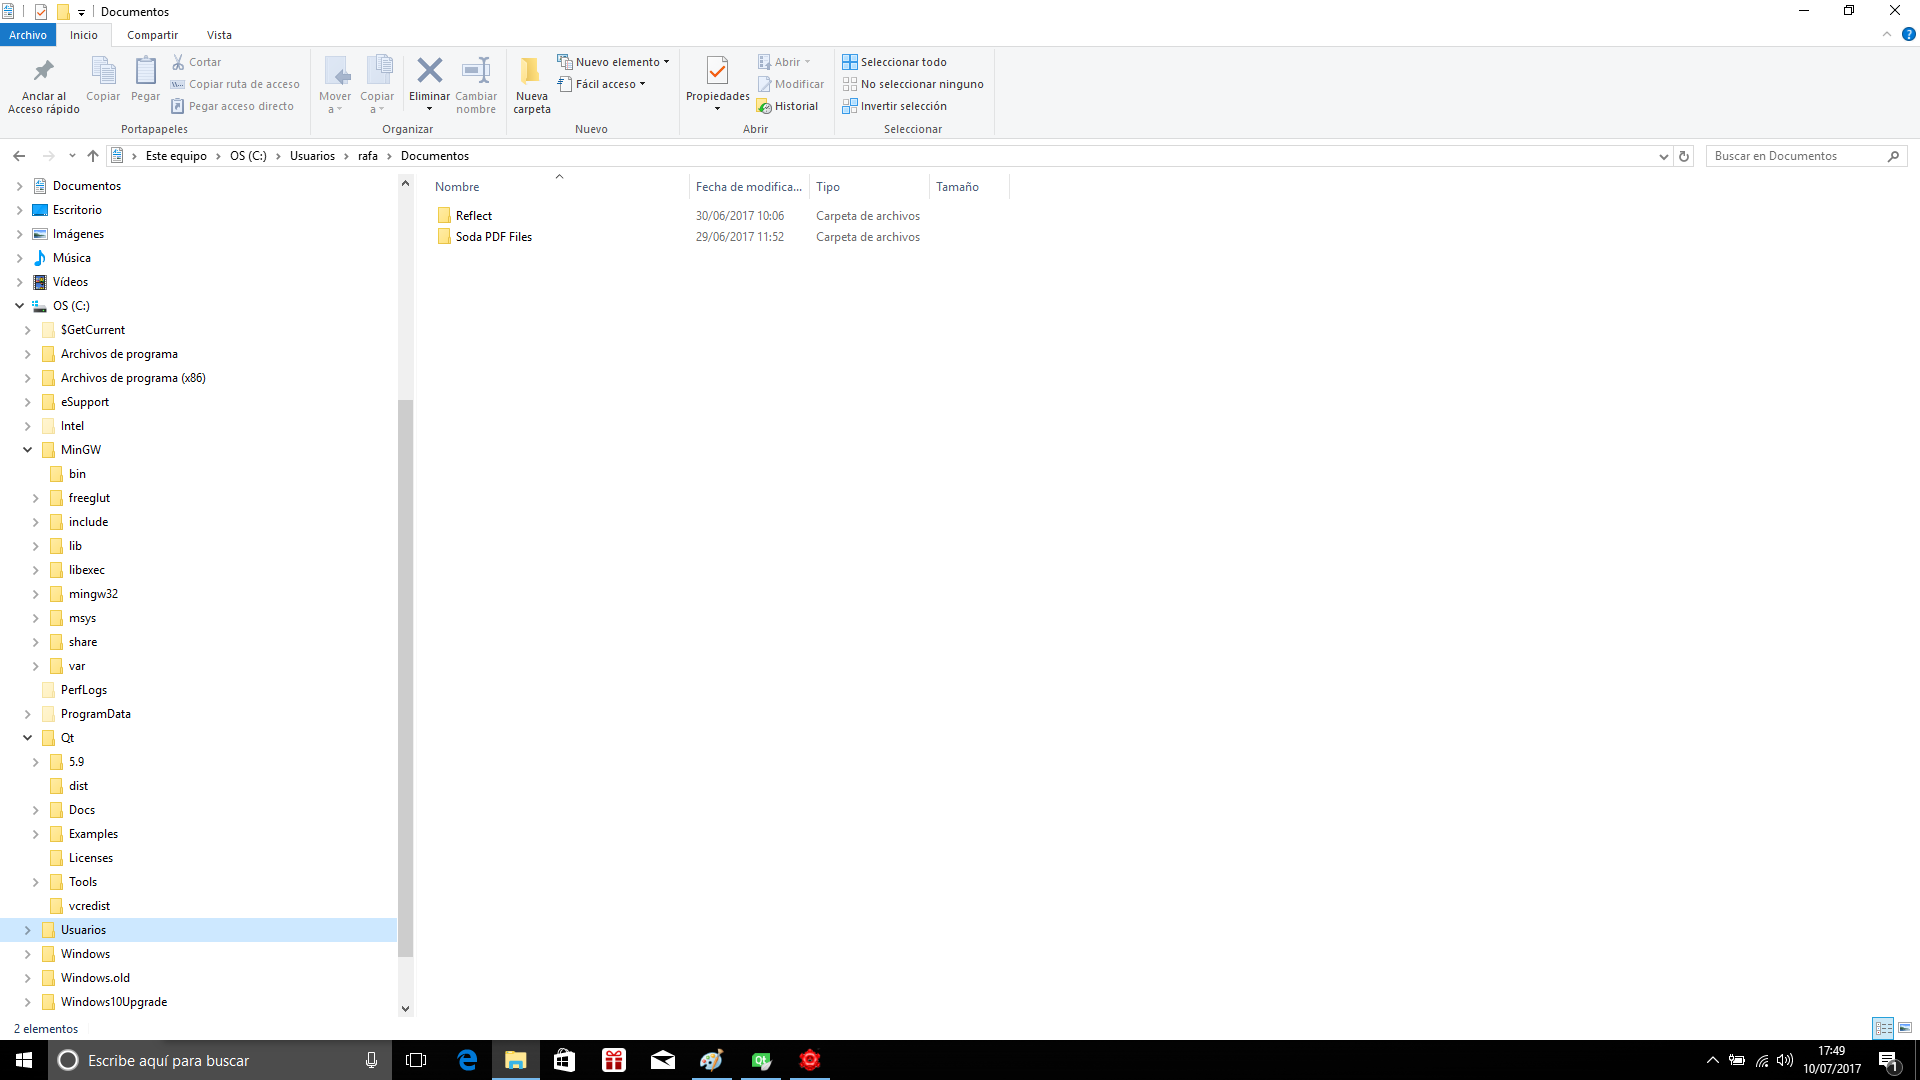
\includegraphics[width=6.5cm]{fig1.png}
\vspace*{1mm}
\caption{\small Software for MSWindows installer of DAMQT \label{fig:1}}
\end{center}
\end{figure}
\end{minipage}
\begin{minipage}{0.5\linewidth}
\begin{figure}[H]
\begin{center}
\vspace*{-4mm}
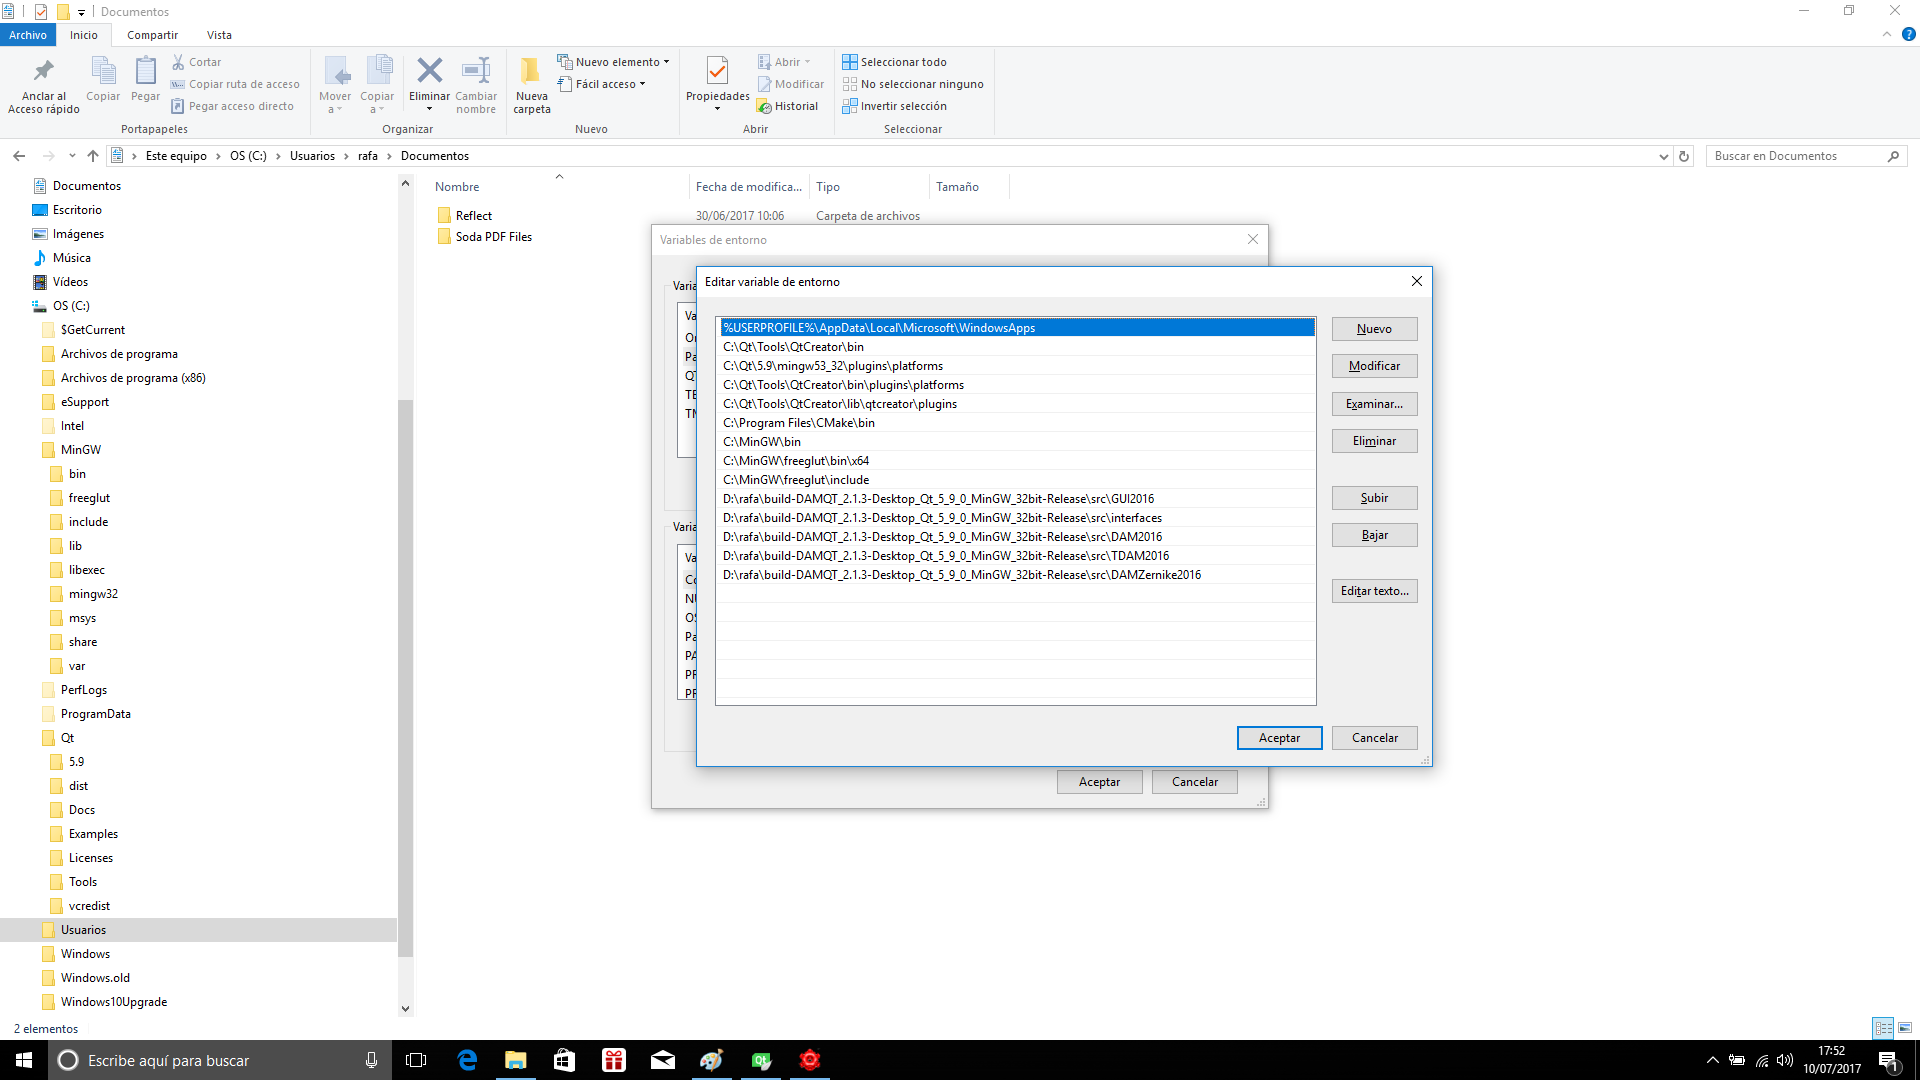
\includegraphics[width=6.5cm]{fig2.png}
\caption{\small \texttt{PATH} settings for Qt creator \label{fig:2}}
\end{center}
\end{figure}
\end{minipage}

To get the Qt creator working properly, some directories must be accessible.
This can be achieved, for instance, by adding them to the environment variable \texttt{PATH}.
The \texttt{PATH} settings shown in fig \ref{fig:2} are sufficient to do the job. 


%
DAMQT package can be installed by unzipping the corresponding tarball (which is delivered compressed with \texttt{gzip}).
This can be done with any suitable tool or, alternatively, with Mingw32. In this case, open
a MSYS console (which will ba available in the \texttt{MinGW/msys/1.0} folder),
navigate to the place where you want to deploy the package and run the command:

\texttt{tar vxzf DAMQTtarball.gz} \\ \\
%
where \texttt{DAMQTtarball} stands for the name of the tarball to be deployed including its full path.
The package will be deployed in a folder named \texttt{DAMQT\_2.1.3}.

\section{Bulding the project with Qt creator}

Once the software is installed, the corresponding executables can be generated using Qt creator.
To do this, launch Qt creator and you will get the {\it Welcome} page, similar to that shown in fig \ref{fig:3}.

\begin{minipage}{0.5\linewidth}
\begin{figure}[H]
\begin{center}
\vspace*{-3mm}
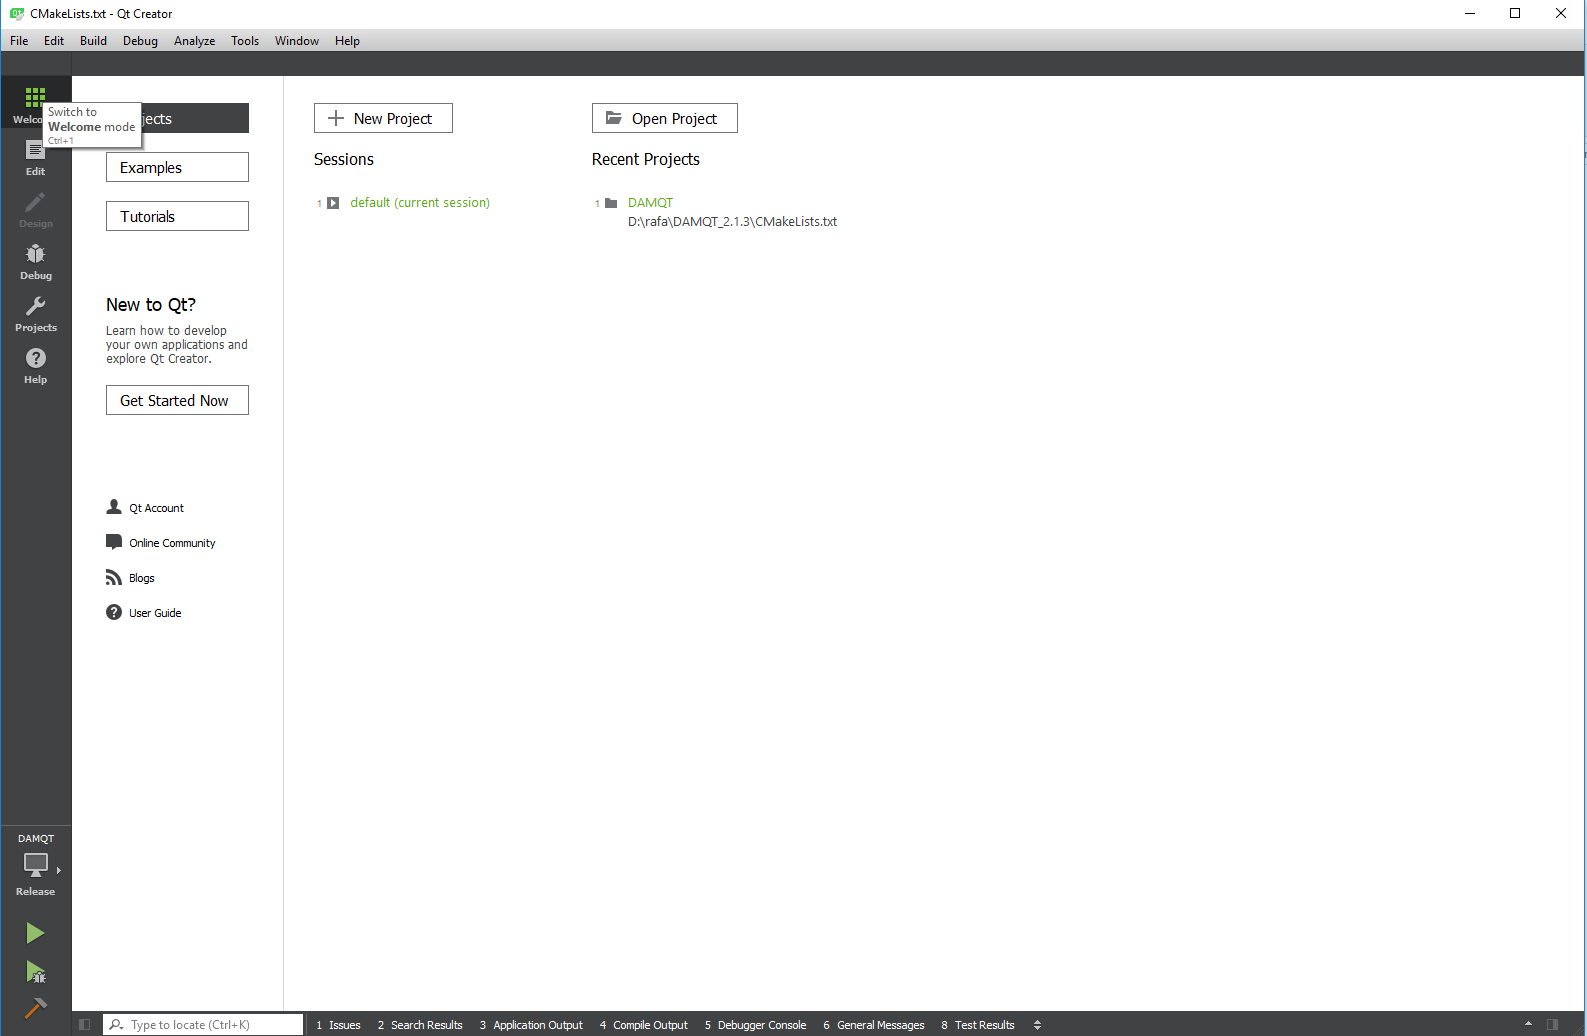
\includegraphics[width=5.5cm]{fig3.png}
\vspace*{-1mm}
\caption{\small Qt creator {\it Welcome} page\label{fig:3}}
\end{center}
\end{figure}
\end{minipage}
\begin{minipage}{0.5\linewidth}
\begin{figure}[H]
\begin{center}
\vspace*{-3mm}
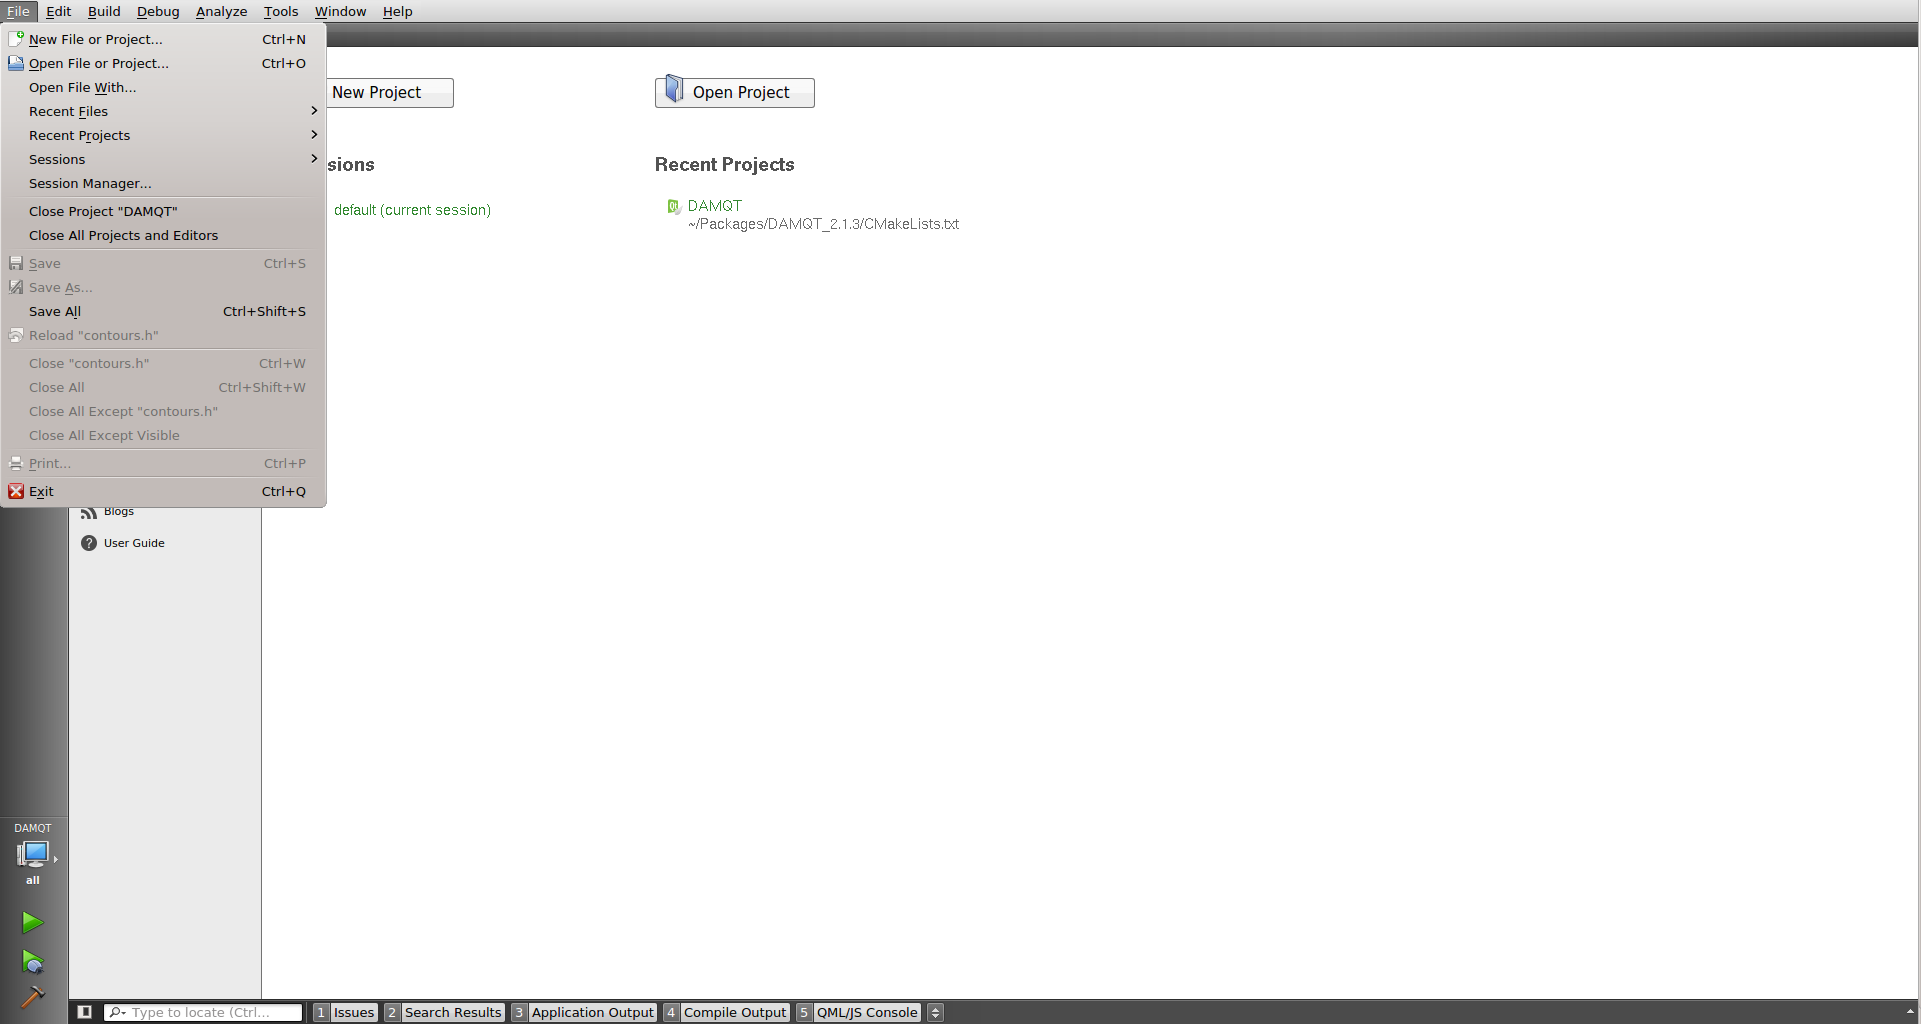
\includegraphics[width=6.5cm]{fig4.png}
\caption{\small {\it File} menu \label{fig:4}}
\end{center}
\end{figure}
\end{minipage}


Within Qt creator, the DAMQT project can be built using \texttt{cmake}. For this purpose, click on the
upper left option {\it File} in the toolbar and a menu will be displayed as shown in fig \ref{fig:4}.
Push the option {\it Open File or Project} and a navigator will appear (see fig \ref{fig:5}).
Navigate to the home directory of the application and select the
{\it CMakeLists.txt}. Selecting a {\it CMakeLists.txt} file triggers \texttt{cmake} utility. Running \texttt{cmake} 
directly, it would complain of undefined environment variables. It also may eventually complain that \texttt{cmake} 
is not available. For these reasons, it is better to decline building the project for the moment and to make some settings before,
using the {\it Projects} option in the left vertical menu. Pressing on it, a screen appears like that shown in fig \ref{fig:6}.

\begin{minipage}{0.5\linewidth}
\begin{figure}[H]
\begin{center}
% \vspace*{-3mm}
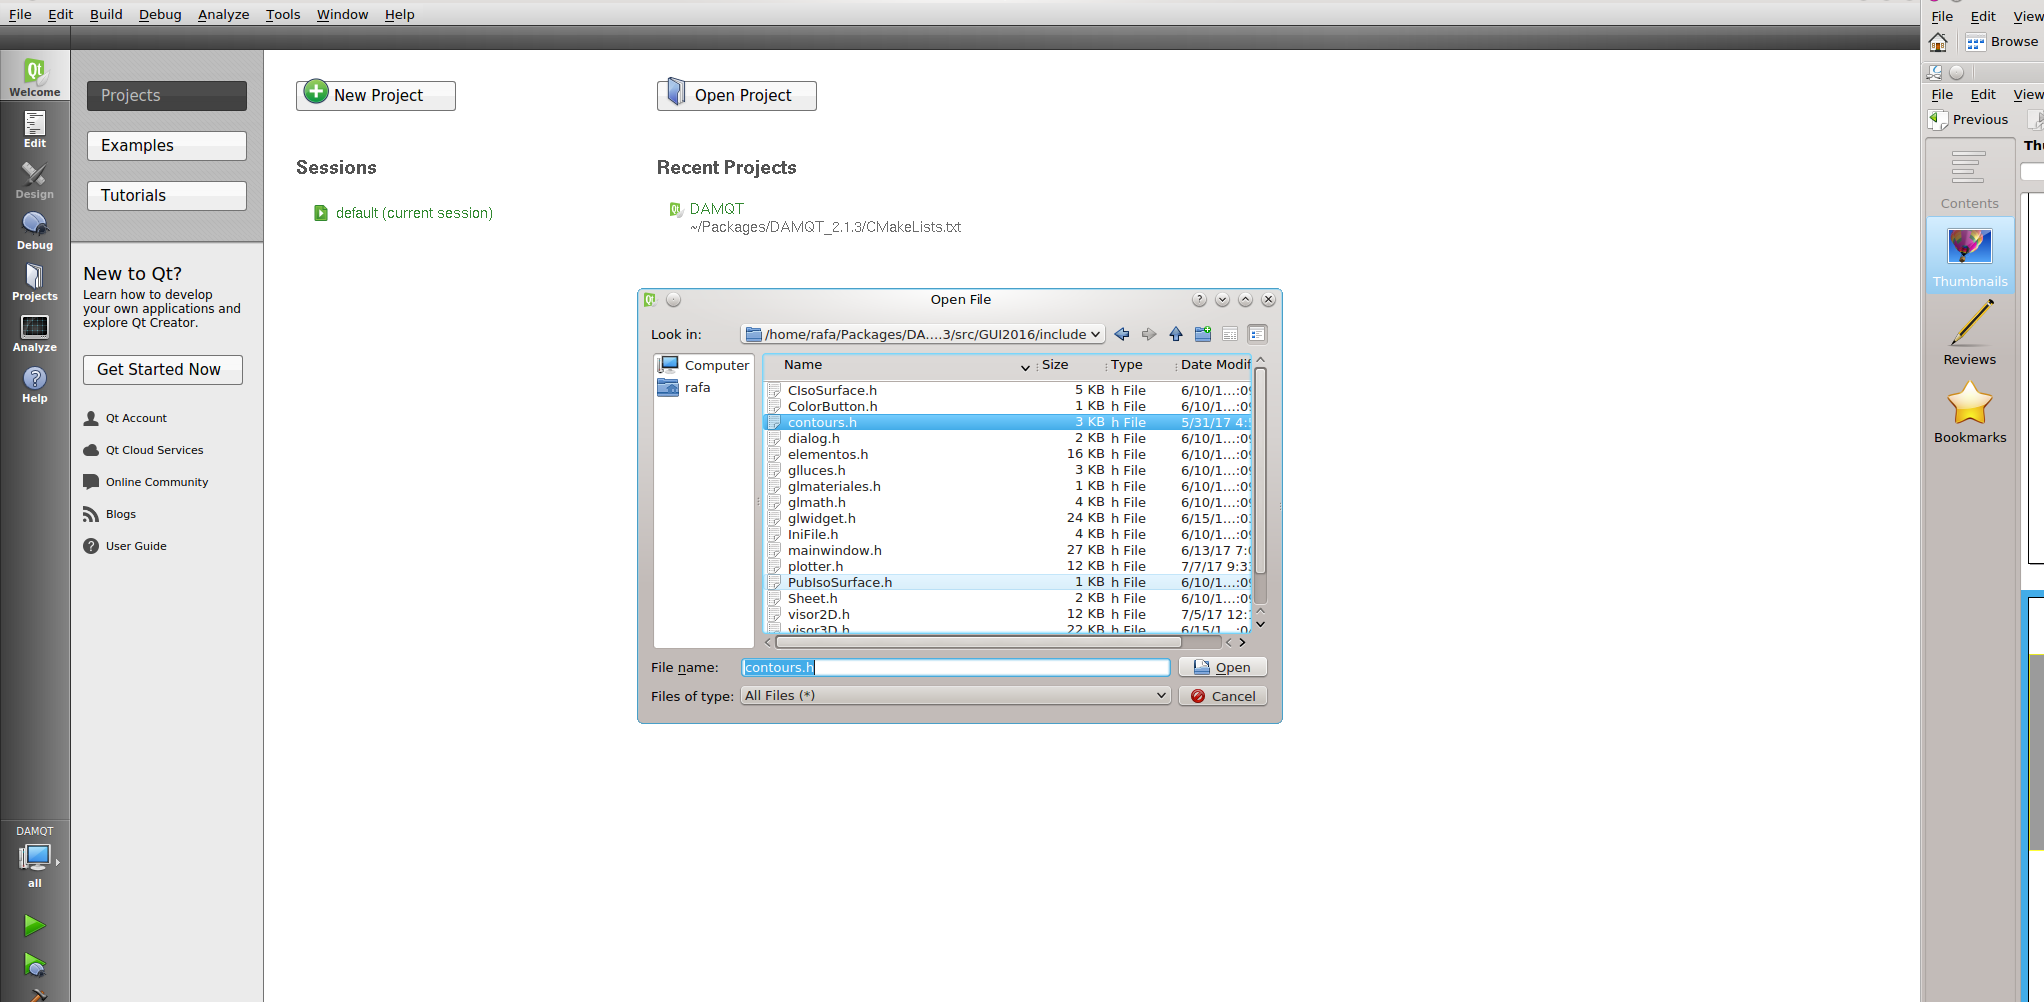
\includegraphics[width=5.5cm]{fig5.png}
\vspace*{-1mm}
\caption{\small  \label{fig:5}}
\end{center}
\end{figure}
\end{minipage}
\begin{minipage}{0.5\linewidth}
\begin{figure}[H]
\begin{center}
% \vspace*{-3mm}
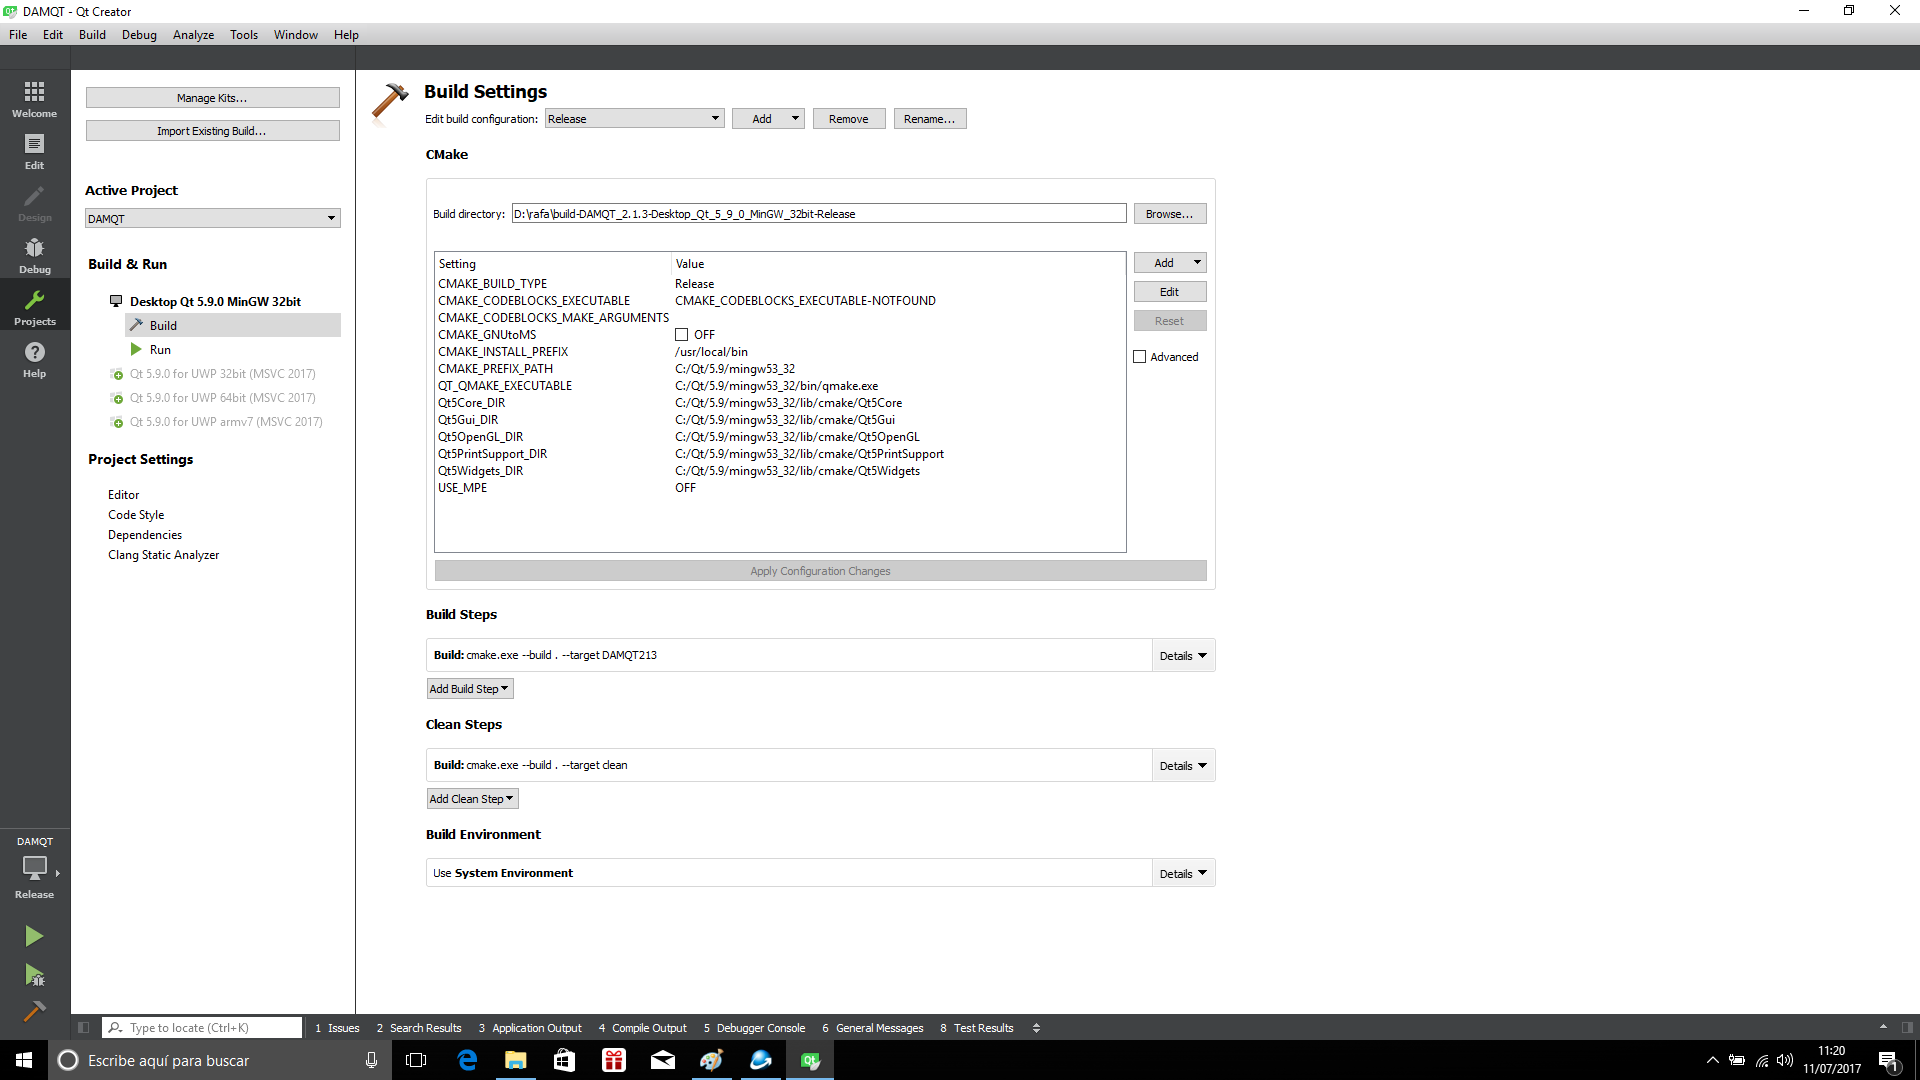
\includegraphics[width=5.5cm]{fig6.png}
\vspace*{-1mm}
\caption{\small  \label{fig:6}}
\end{center}
\end{figure}
\end{minipage}

In this screen, a suitable directory for building the project should be chosen in the box labeled
{\it Build directory}. A temptative name is proposed, but it can be changed to any other of your preference.
Below that box, another one is opened containing the current settings of some environment variables.
Checking the box labeled as {\it Advanced}, all the meaningful environment variables will appear.
In figs \ref{fig:7} to \ref{fig:12}, suitable settings of the variables are shown, according to the
installation proposed.

\begin{minipage}{0.5\linewidth}
\begin{figure}[H]
\begin{center}
% \vspace*{-3mm}
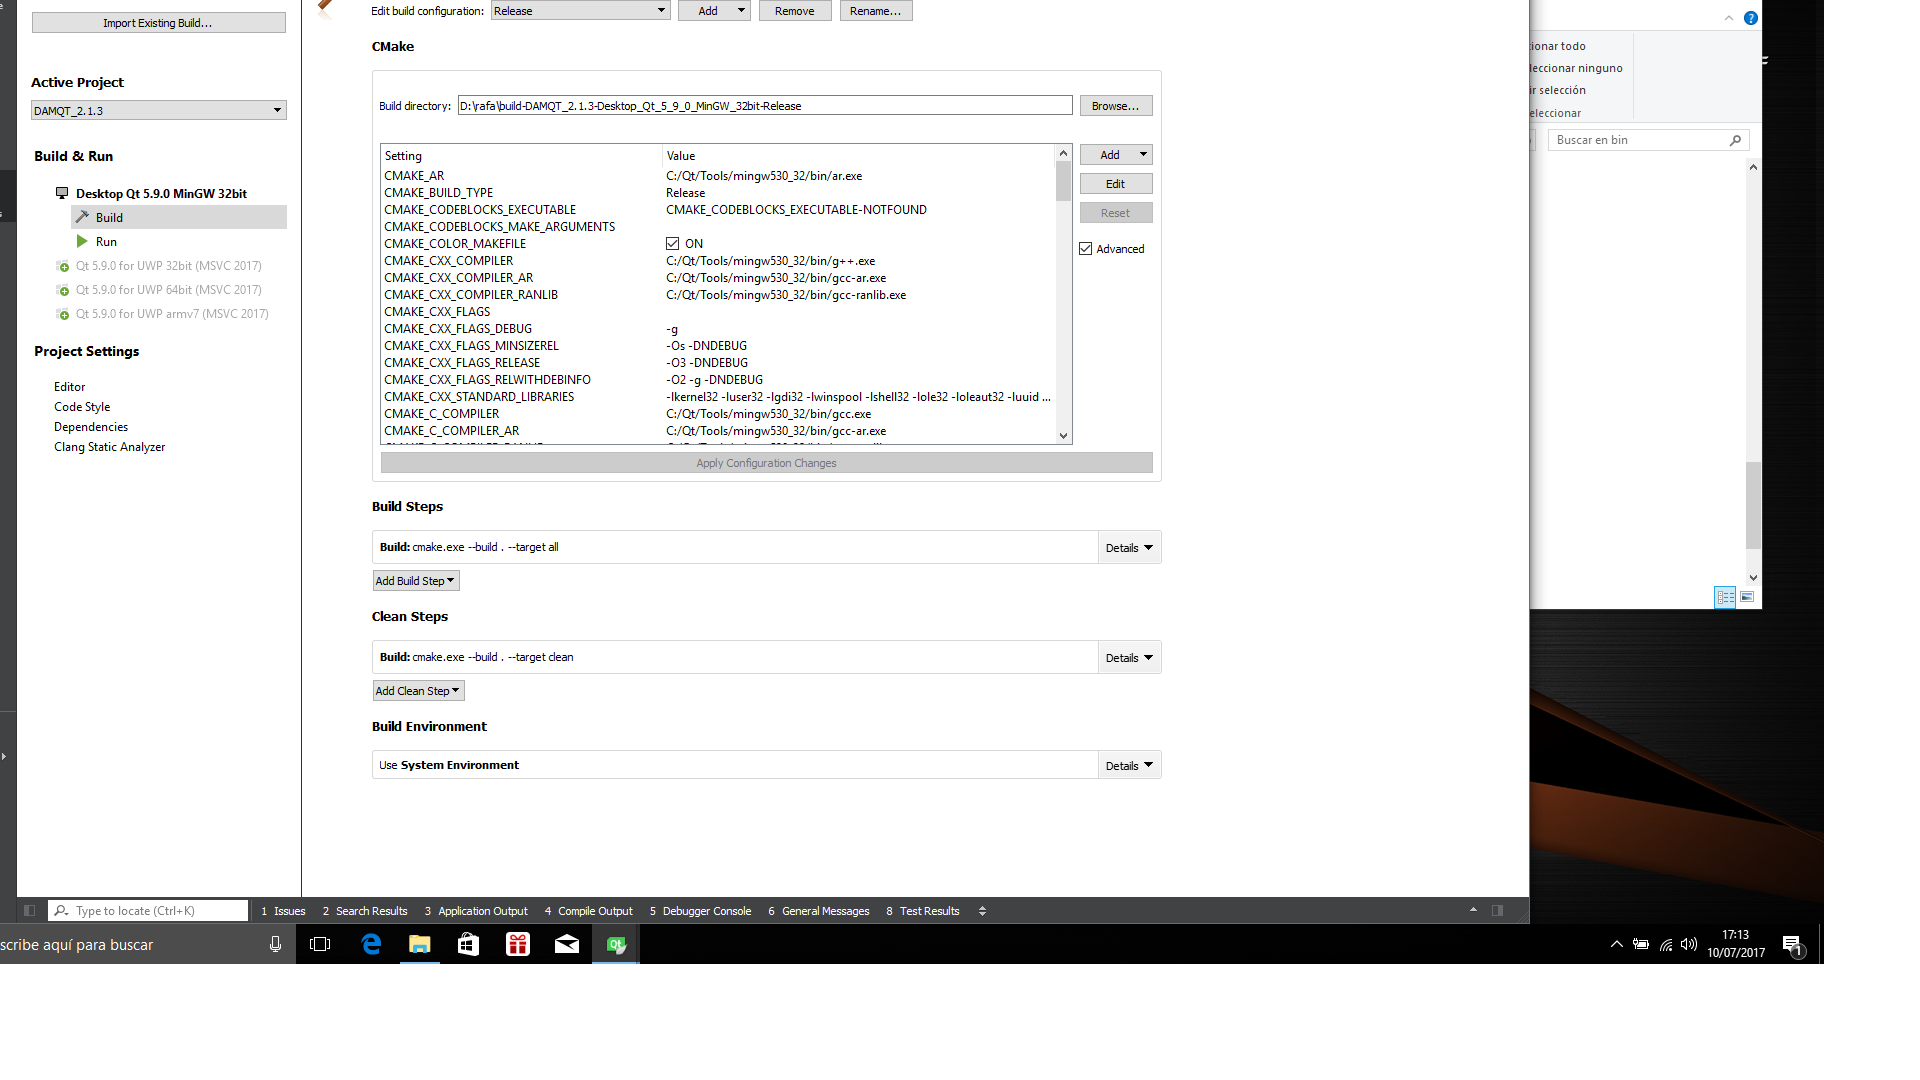
\includegraphics[width=5.5cm]{fig7.png}
\vspace*{-1mm}
\caption{\small  \label{fig:7}}
\end{center}
\end{figure}
\end{minipage}
\begin{minipage}{0.5\linewidth}
\begin{figure}[H]
\begin{center}
% \vspace*{-3mm}
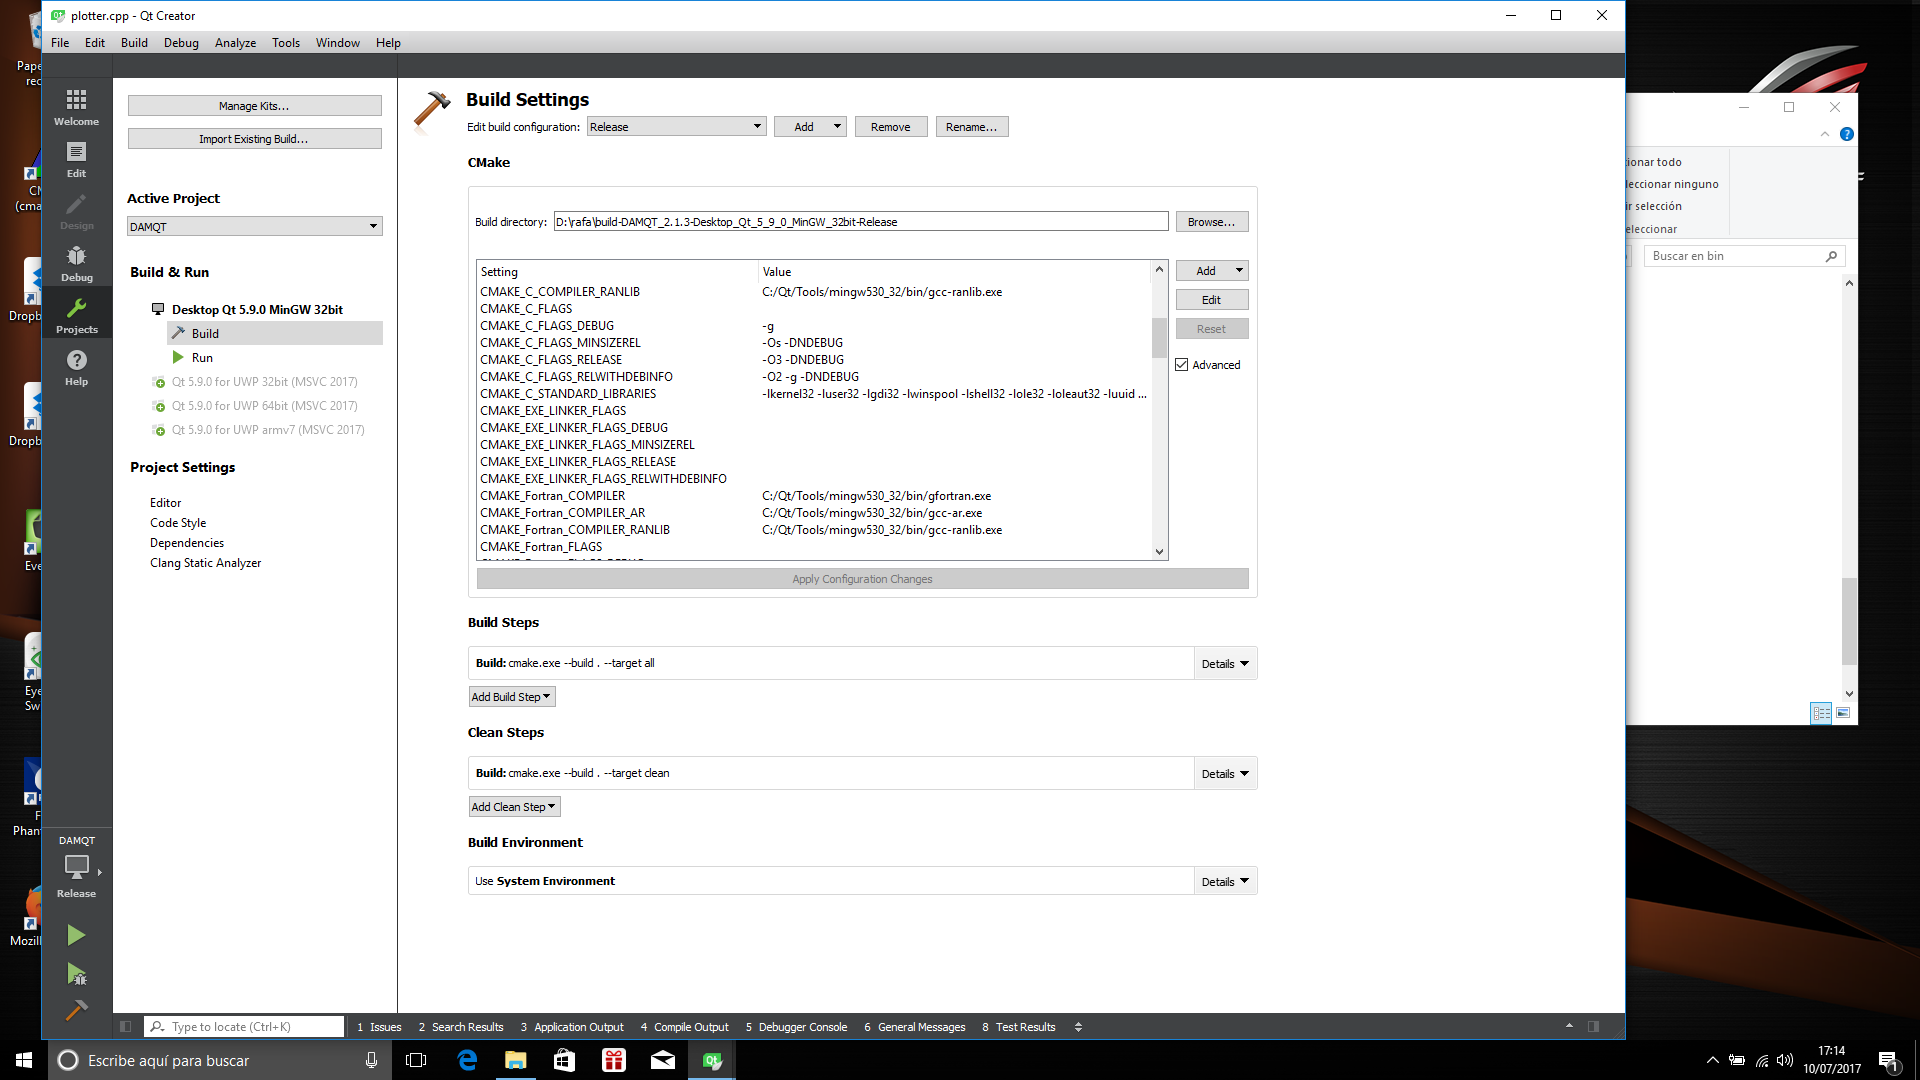
\includegraphics[width=5.5cm]{fig8.png}
\vspace*{-1mm}
\caption{\small  \label{fig:8}}
\end{center}
\end{figure}
\end{minipage}

\begin{minipage}{0.5\linewidth}
\begin{figure}[H]
\begin{center}
% \vspace*{-3mm}
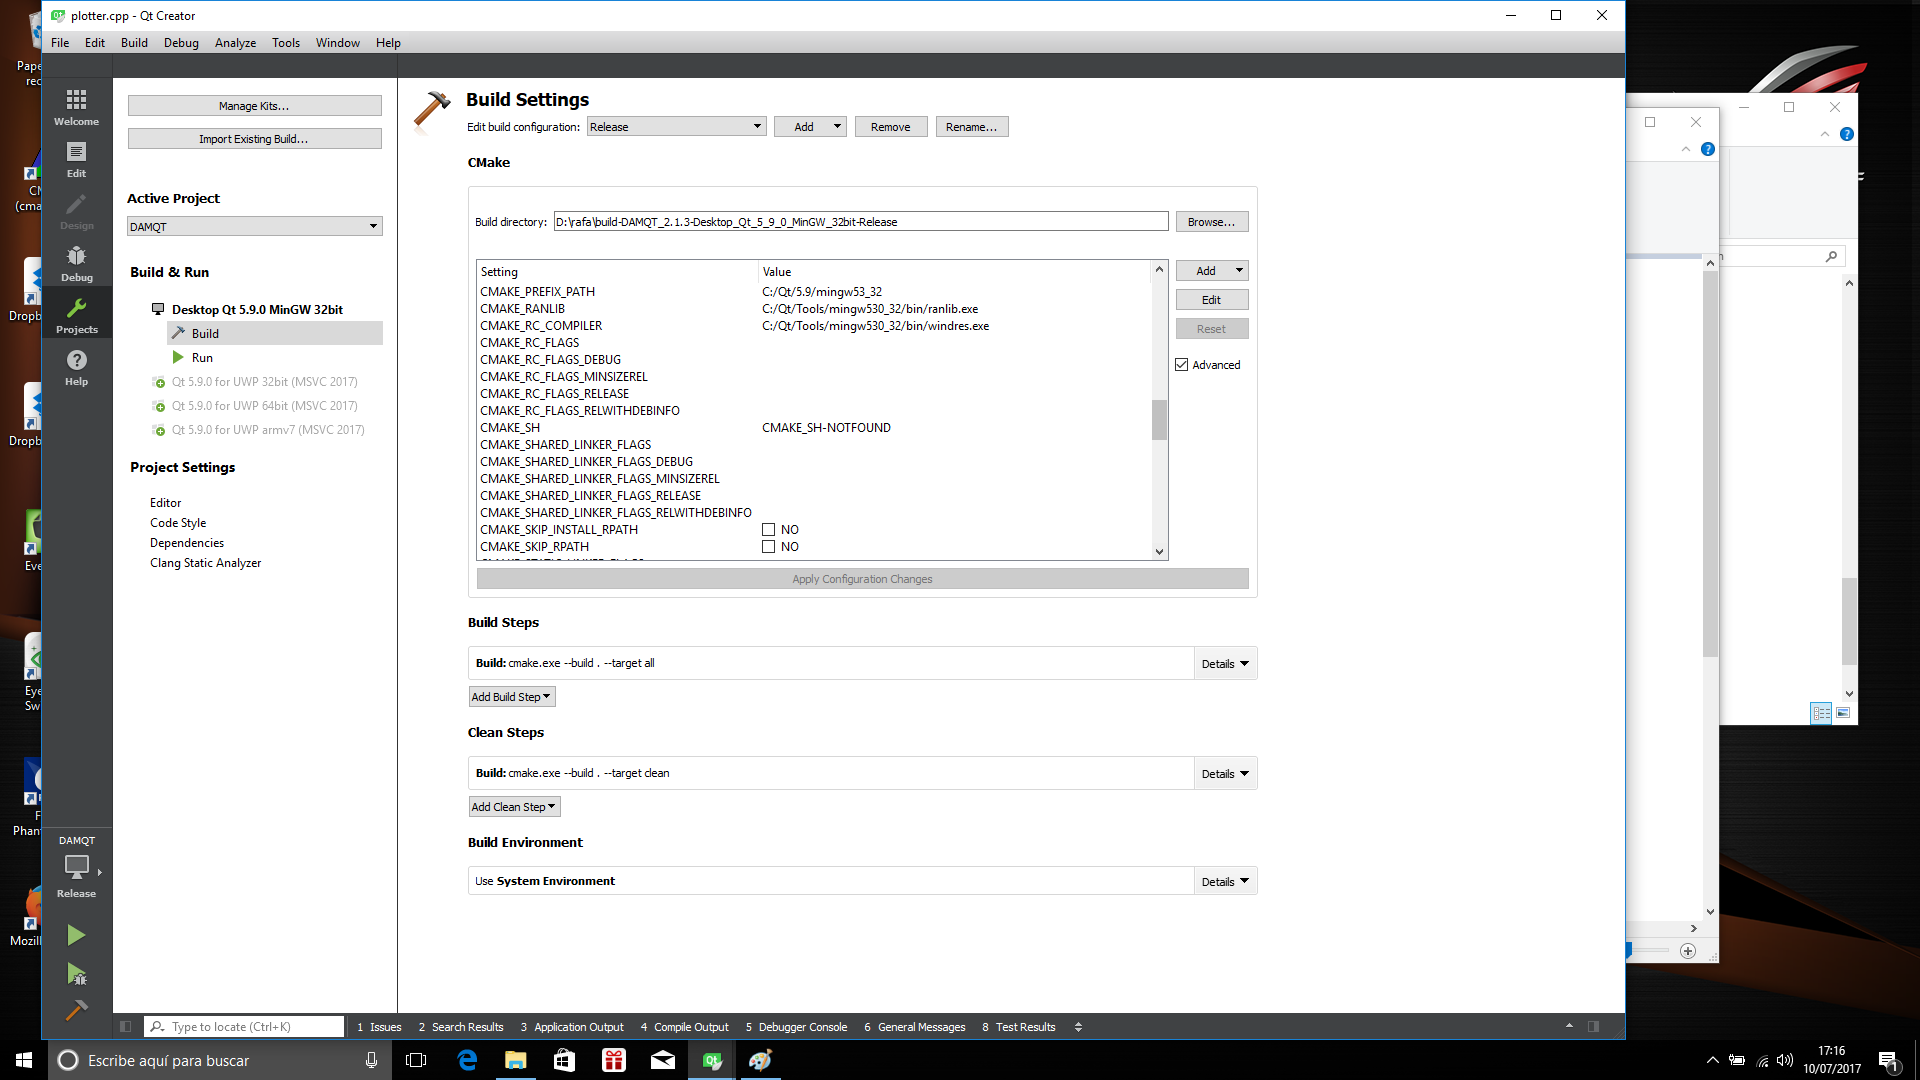
\includegraphics[width=5.5cm]{fig9.png}
\vspace*{-1mm}
\caption{\small  \label{fig:9}}
\end{center}
\end{figure}
\end{minipage}
\begin{minipage}{0.5\linewidth}
\begin{figure}[H]
\begin{center}
% \vspace*{-3mm}
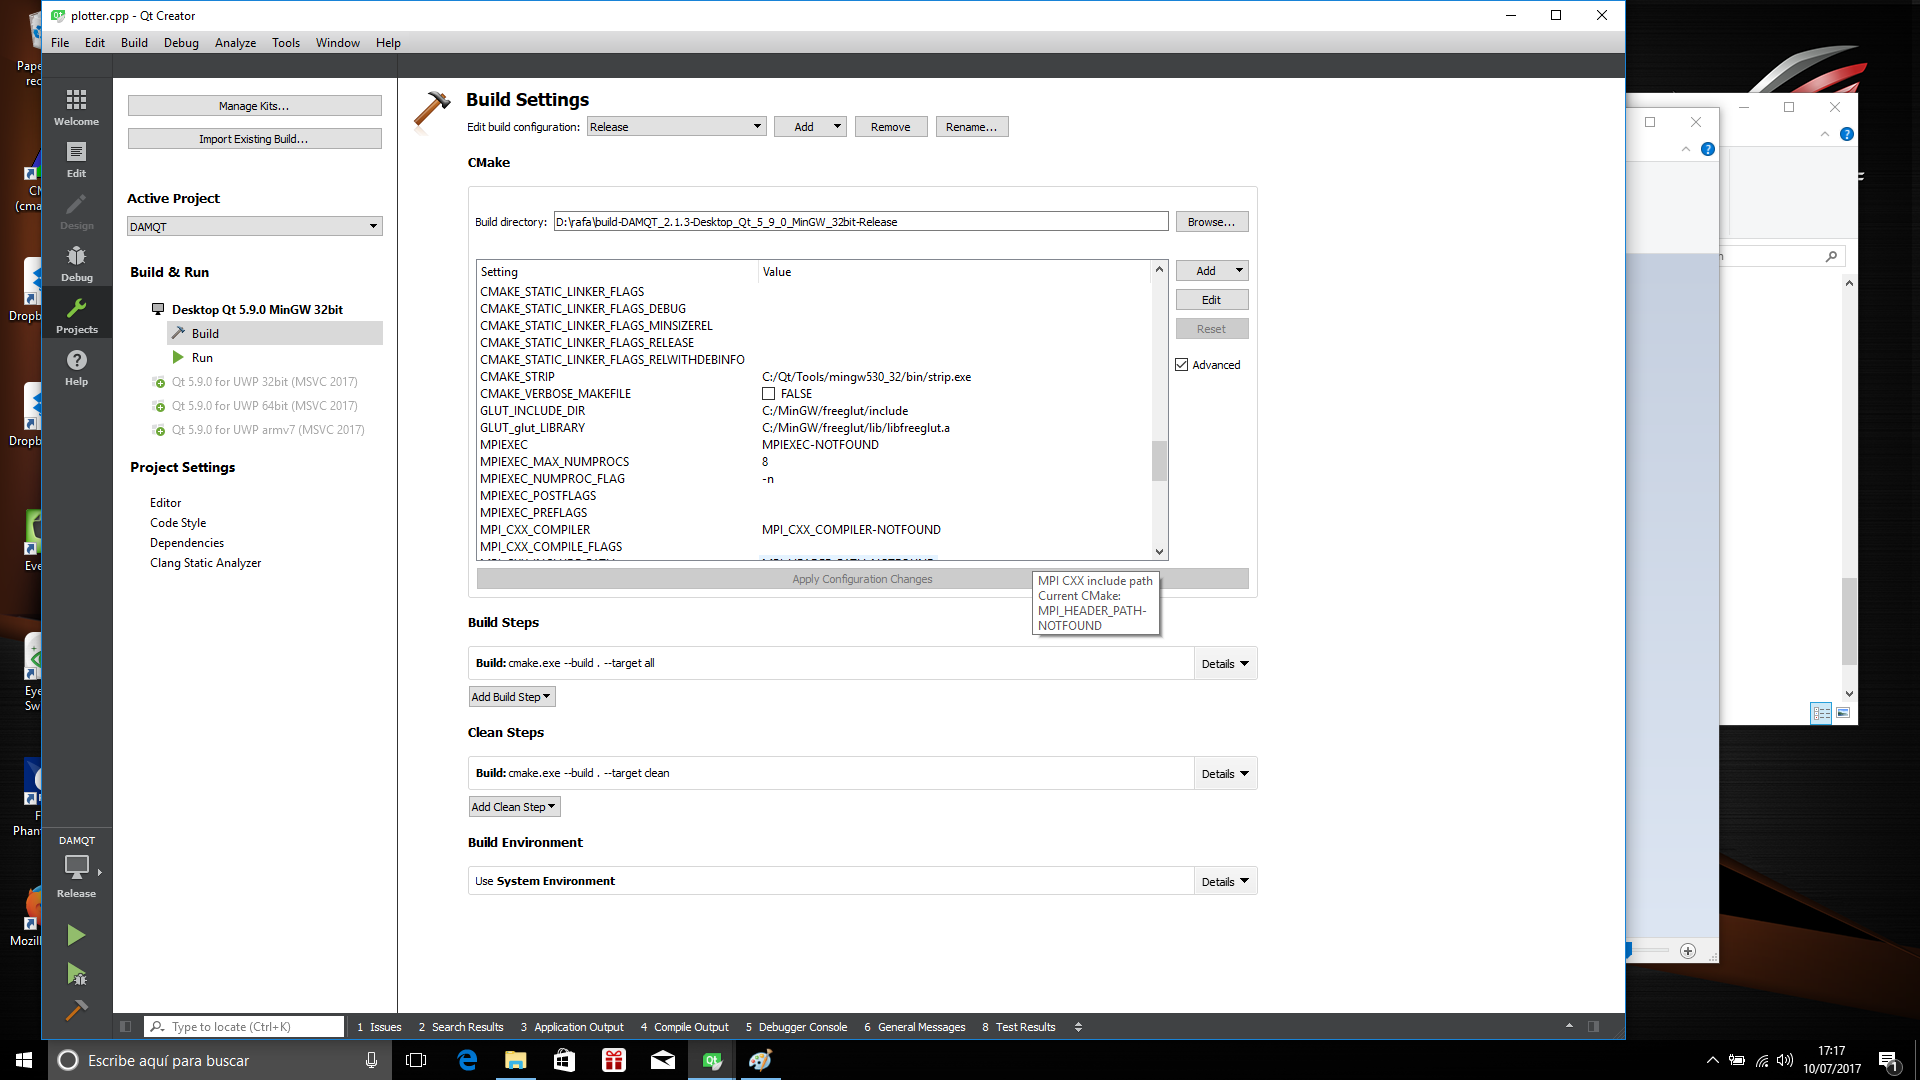
\includegraphics[width=5.5cm]{fig10.png}
\vspace*{-1mm}
\caption{\small  \label{fig:10}}
\end{center}
\end{figure}
\end{minipage}

\begin{minipage}{0.5\linewidth}
\begin{figure}[H]
\begin{center}
% \vspace*{-3mm}
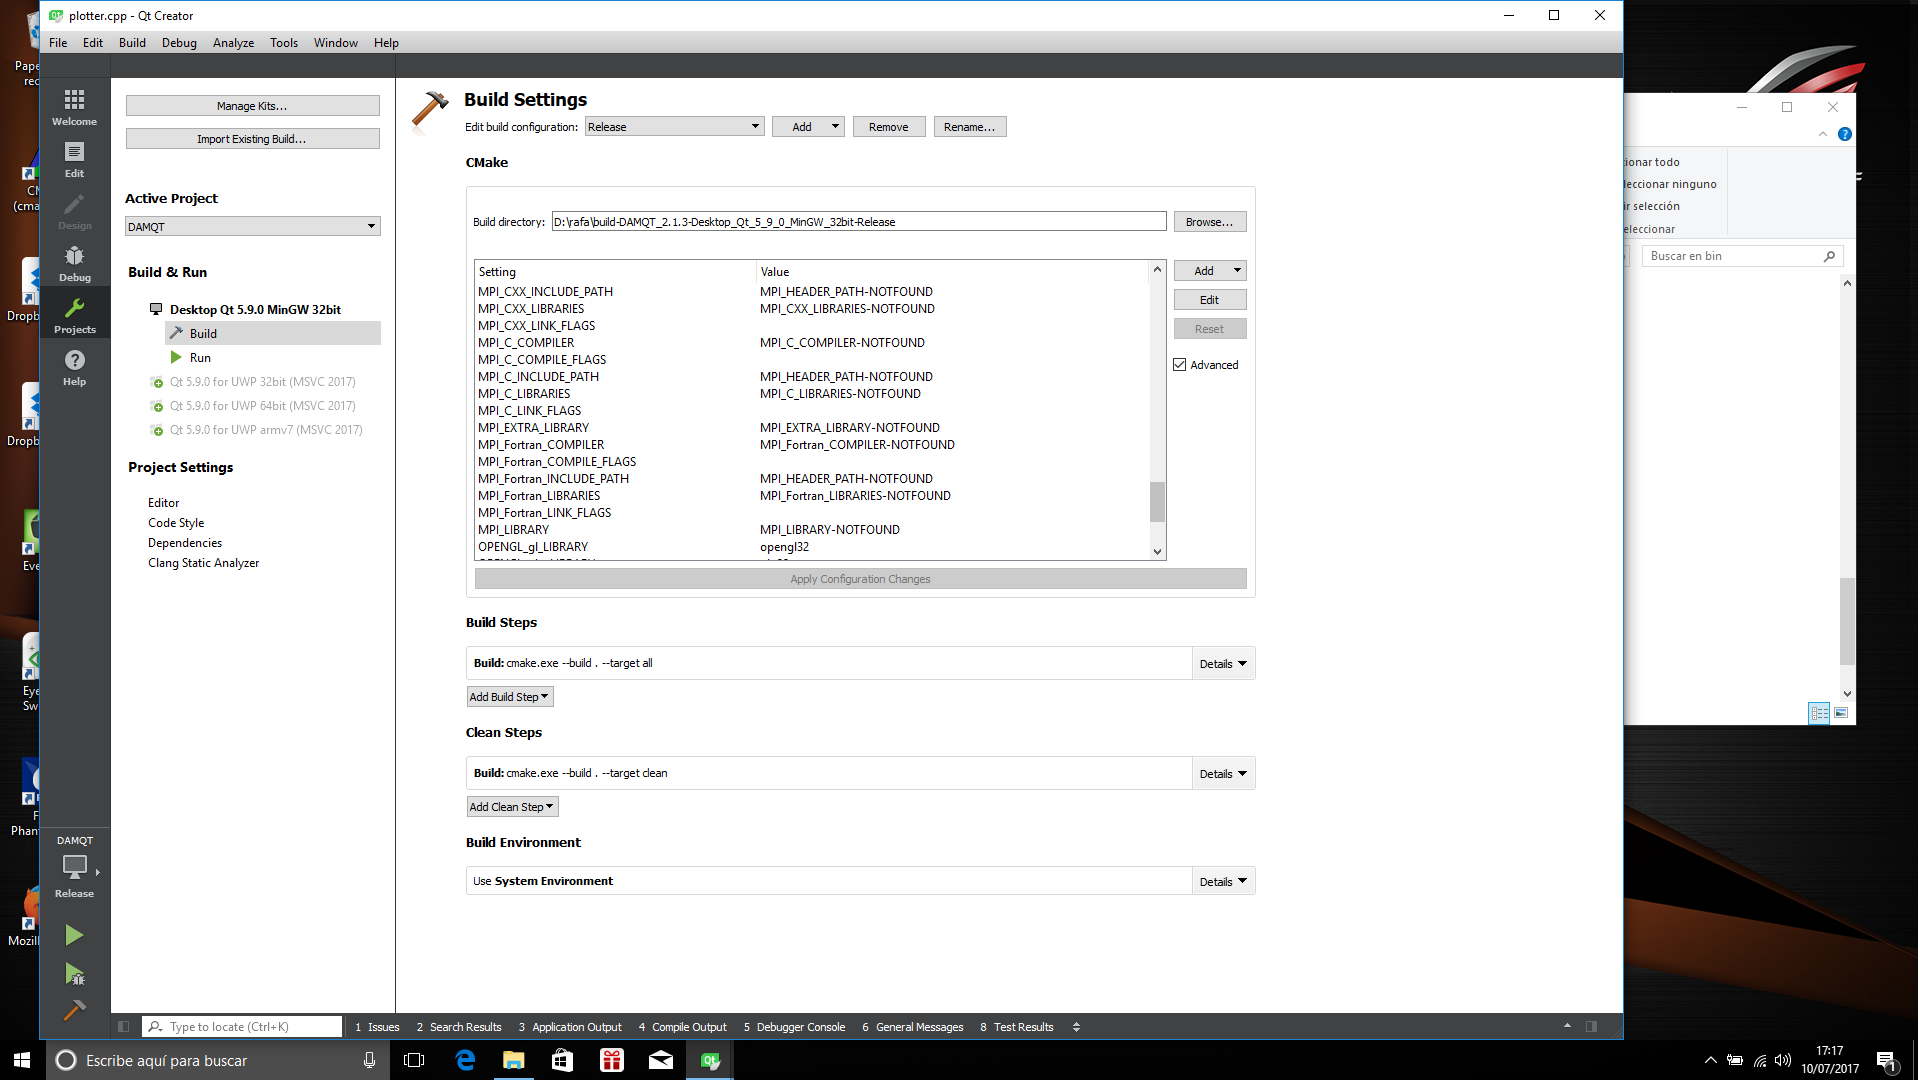
\includegraphics[width=5.5cm]{fig11.png}
\vspace*{-1mm}
\caption{\small  \label{fig:11}}
\end{center}
\end{figure}
\end{minipage}
\begin{minipage}{0.5\linewidth}
\begin{figure}[H]
\begin{center}
% \vspace*{-3mm}
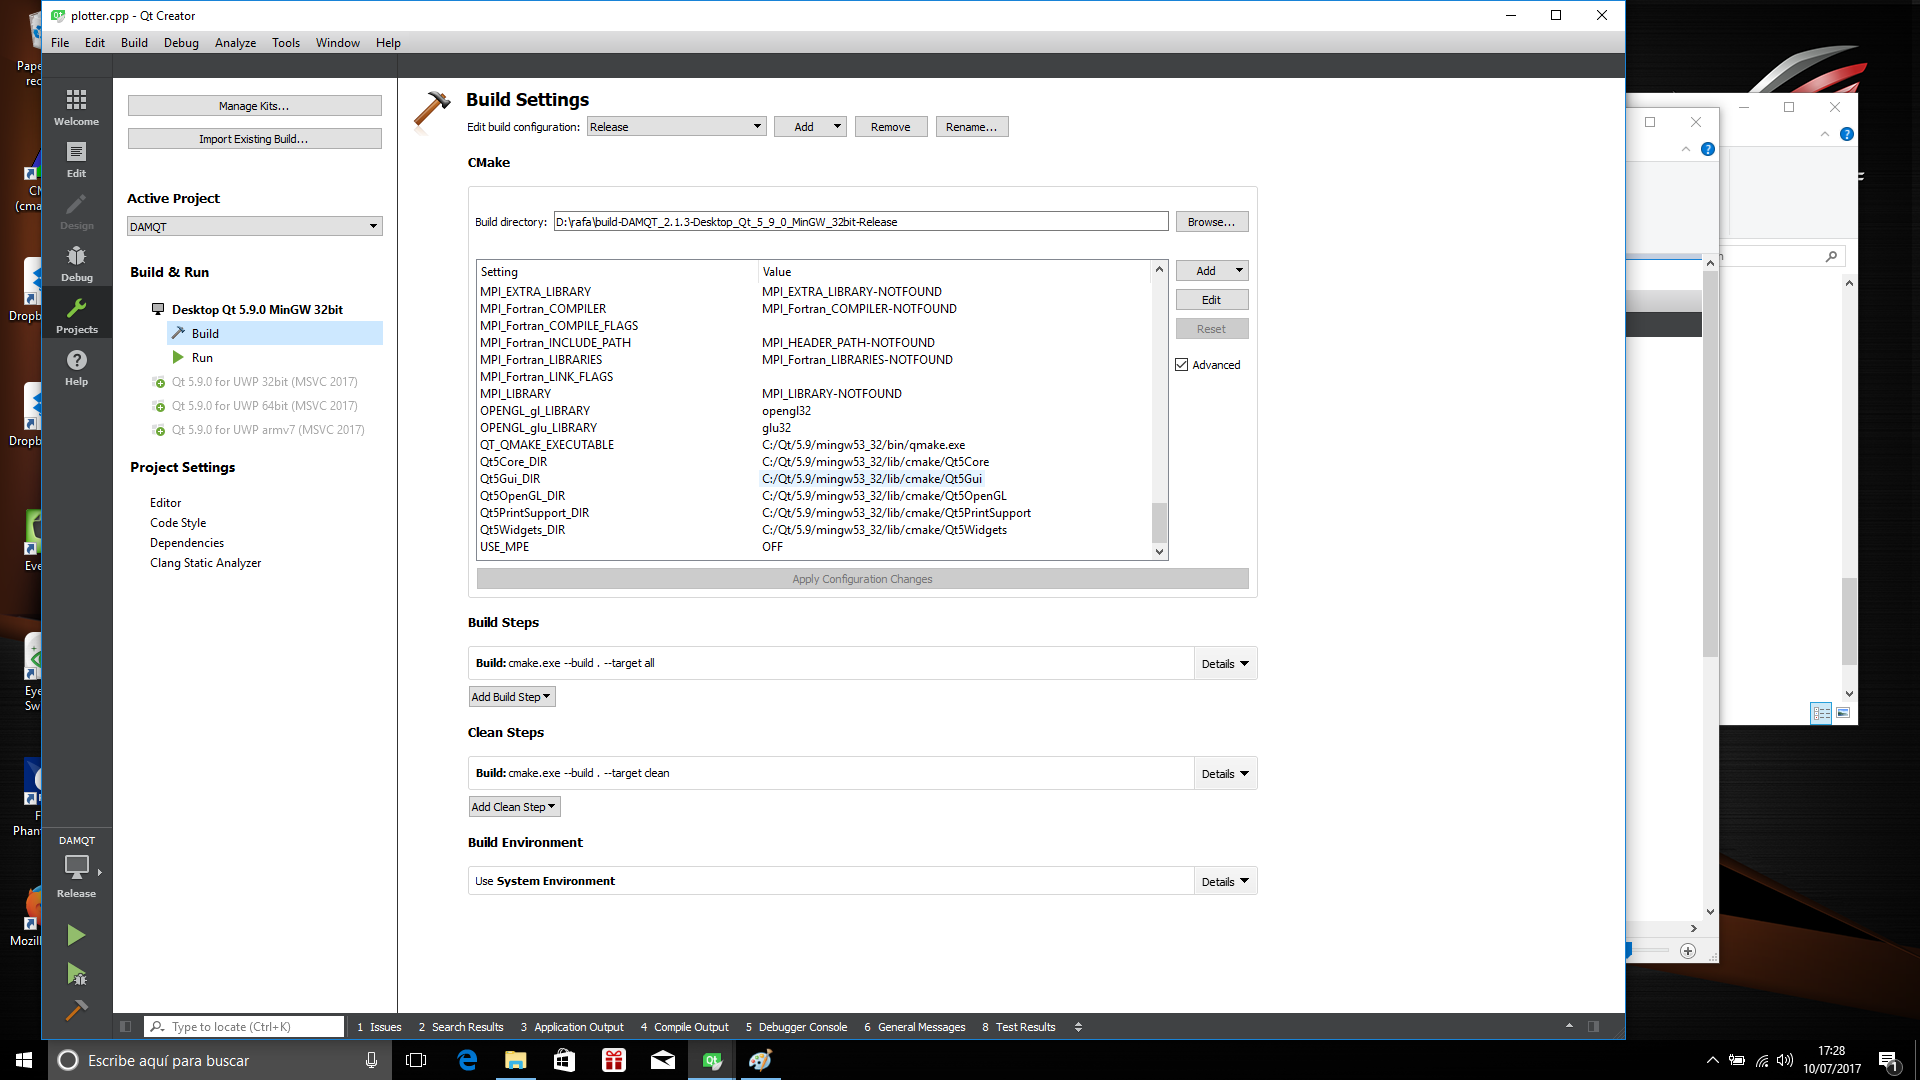
\includegraphics[width=5.5cm]{fig12.png}
\vspace*{-1mm}
\caption{\small  \label{fig:12}}
\end{center}
\end{figure}
\end{minipage}

Next, pressing in the {\it Details} box on the right of {\it Build steps} option, 
a list of possible targets will appear, as fig \ref{fig:13} shows. By default, the {\it all} option is checked.
Uncheck it and check the box corresponding to DAMQT213. Furthermore, {\it Details}
on {\it Build Environment} option will show the environment pertaining variables.
Check that they are correctly set. In particular, check that the \texttt{PATH} variable contains
the paths to the folders commented above.

\begin{minipage}{0.5\linewidth}
\begin{figure}[H]
\begin{center}
% \vspace*{-3mm}
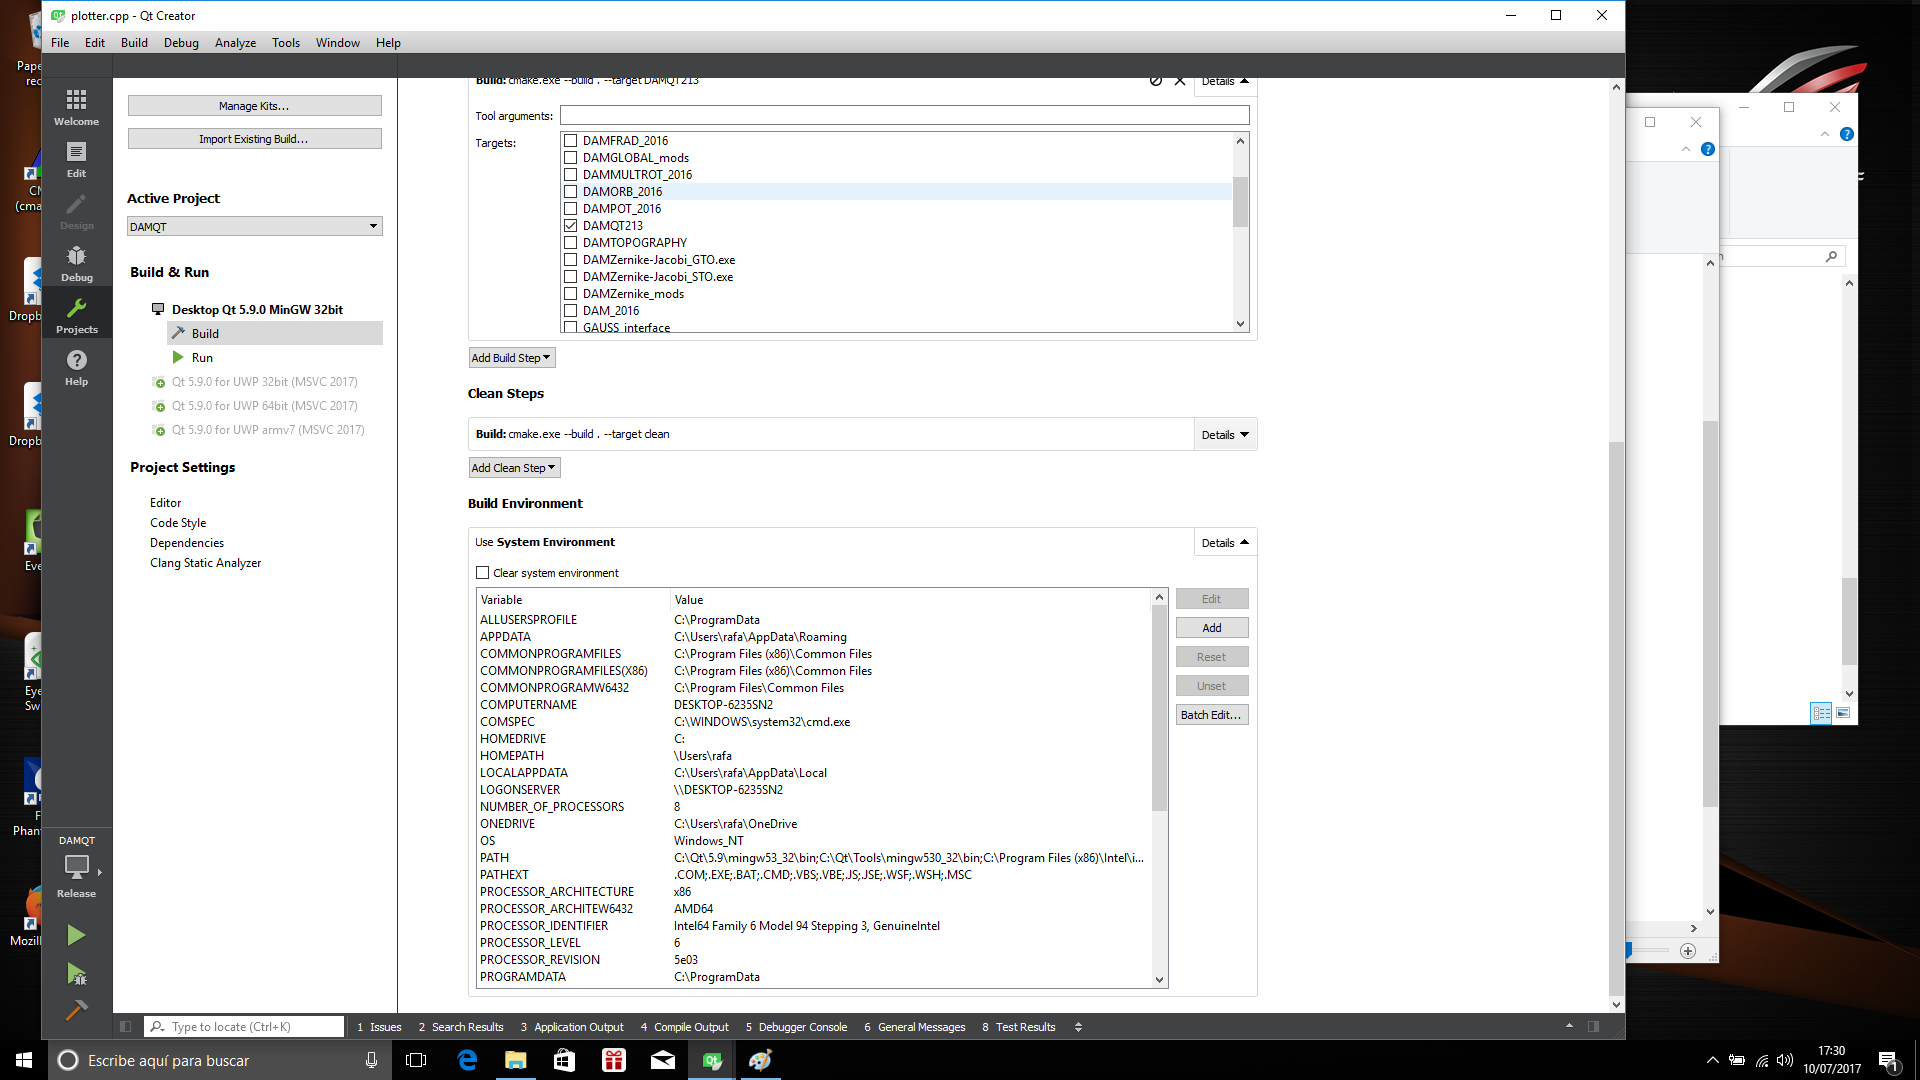
\includegraphics[width=5.5cm]{fig13.png}
\vspace*{-1mm}
\caption{\small  \label{fig:13}}
\end{center}
\end{figure}
\end{minipage}
\begin{minipage}{0.5\linewidth}
\begin{figure}[H]
\begin{center}
% \vspace*{-3mm}
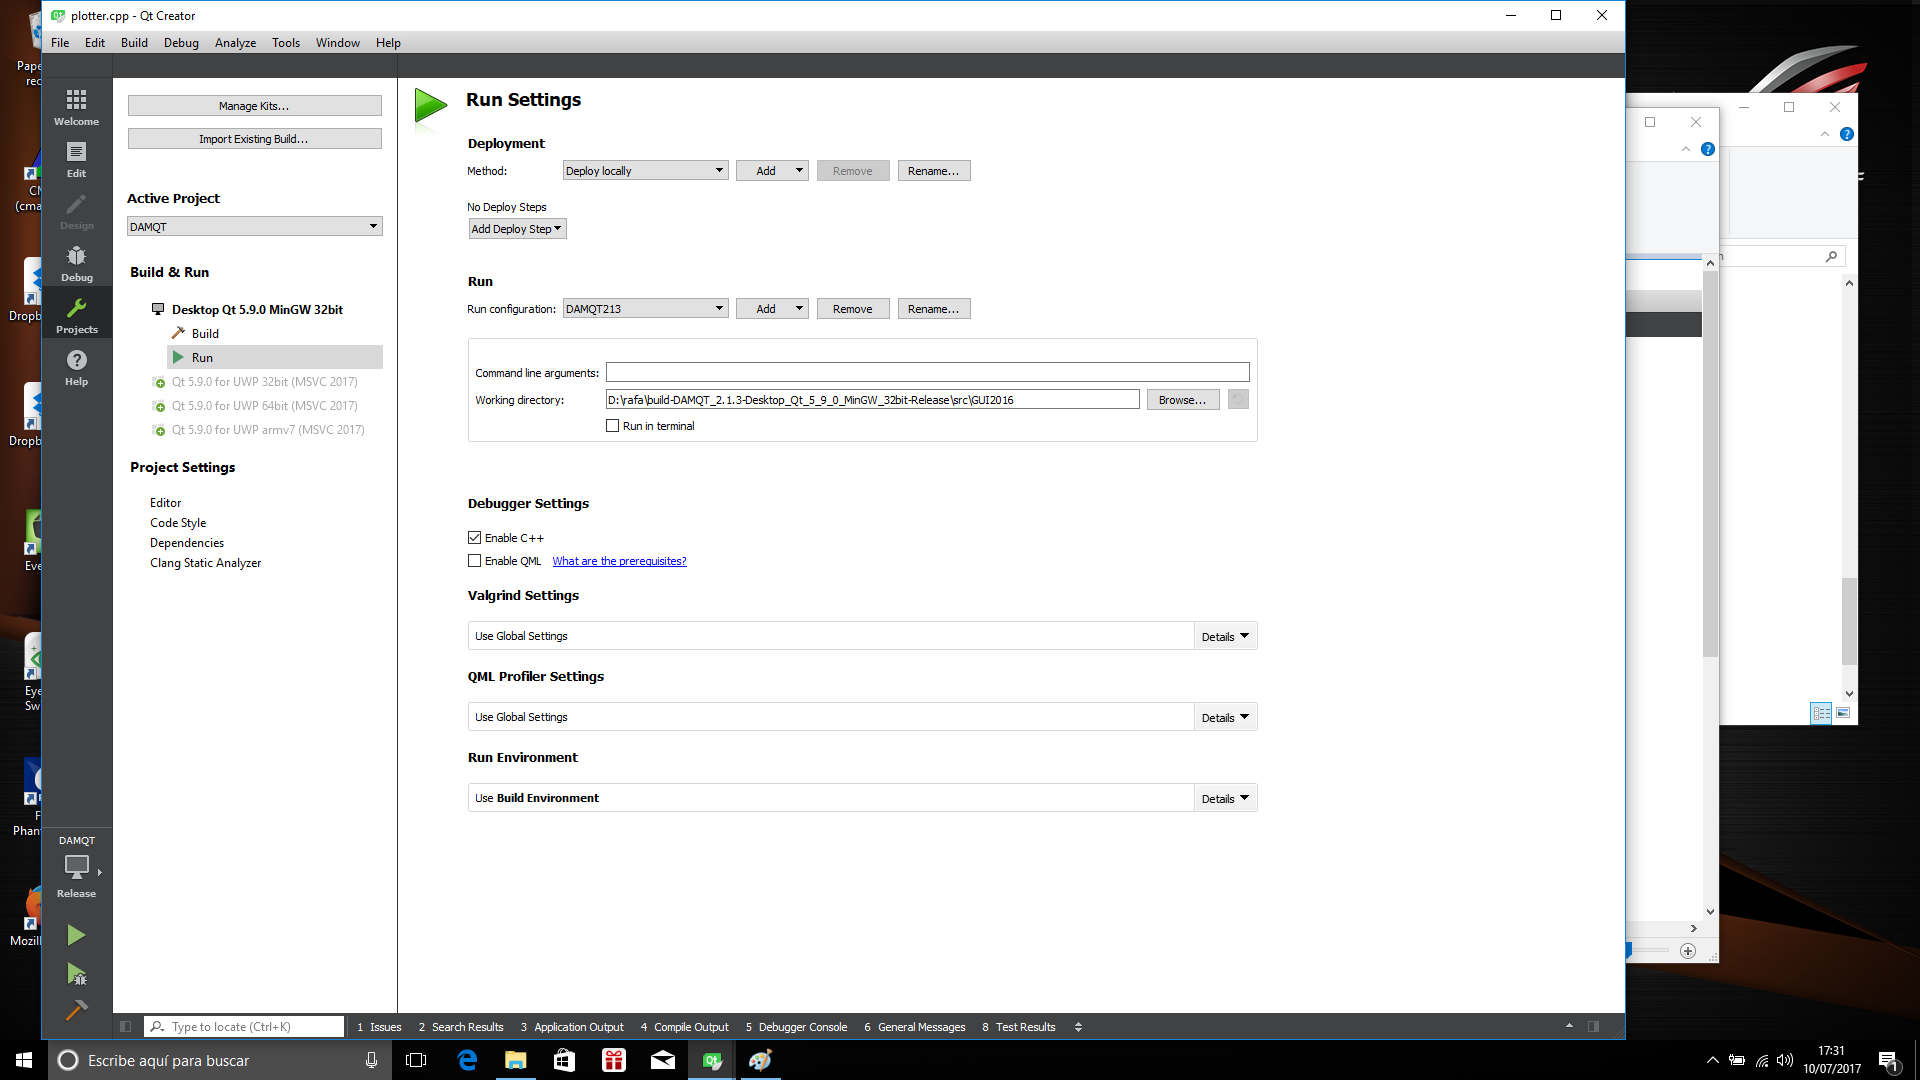
\includegraphics[width=5.5cm]{fig14.png}
\vspace*{-1mm}
\caption{\small  \label{fig:14}}
\end{center}
\end{figure}
\end{minipage}

Selecting the option {\it Run} appearing on te {\it Build and Run} entry on the left, 
a screen will be displayed (see fig \ref{fig:14}) where the {\it Working directory} can be selected among other options.

Pressing in the upper left option {\it Manage kits}, an {\it Options} menu is displayed where important installation settings
are available. As it can be seen in fig \ref{fig:15} there is a menu on the left in which the entry {\it Build and Run}
is very important. Pressing it, the screen gives access to several tabs which deserve comment.

Tab labeled as {\it General} allows us general customization. Default settings are fine, but you can
change them at will. 

{\it Kits} tab (see fig \ref{fig:16}) is important. It lists the different possibilities of project deployment.
{\it Desktop Qt 5.9.0 MinGW 32 bits (default)} shoud be marked as currently chosen 
since we want to build the project with MinGW tools.

\begin{minipage}{0.5\linewidth}
\begin{figure}[H]
\begin{center}
% \vspace*{-3mm}
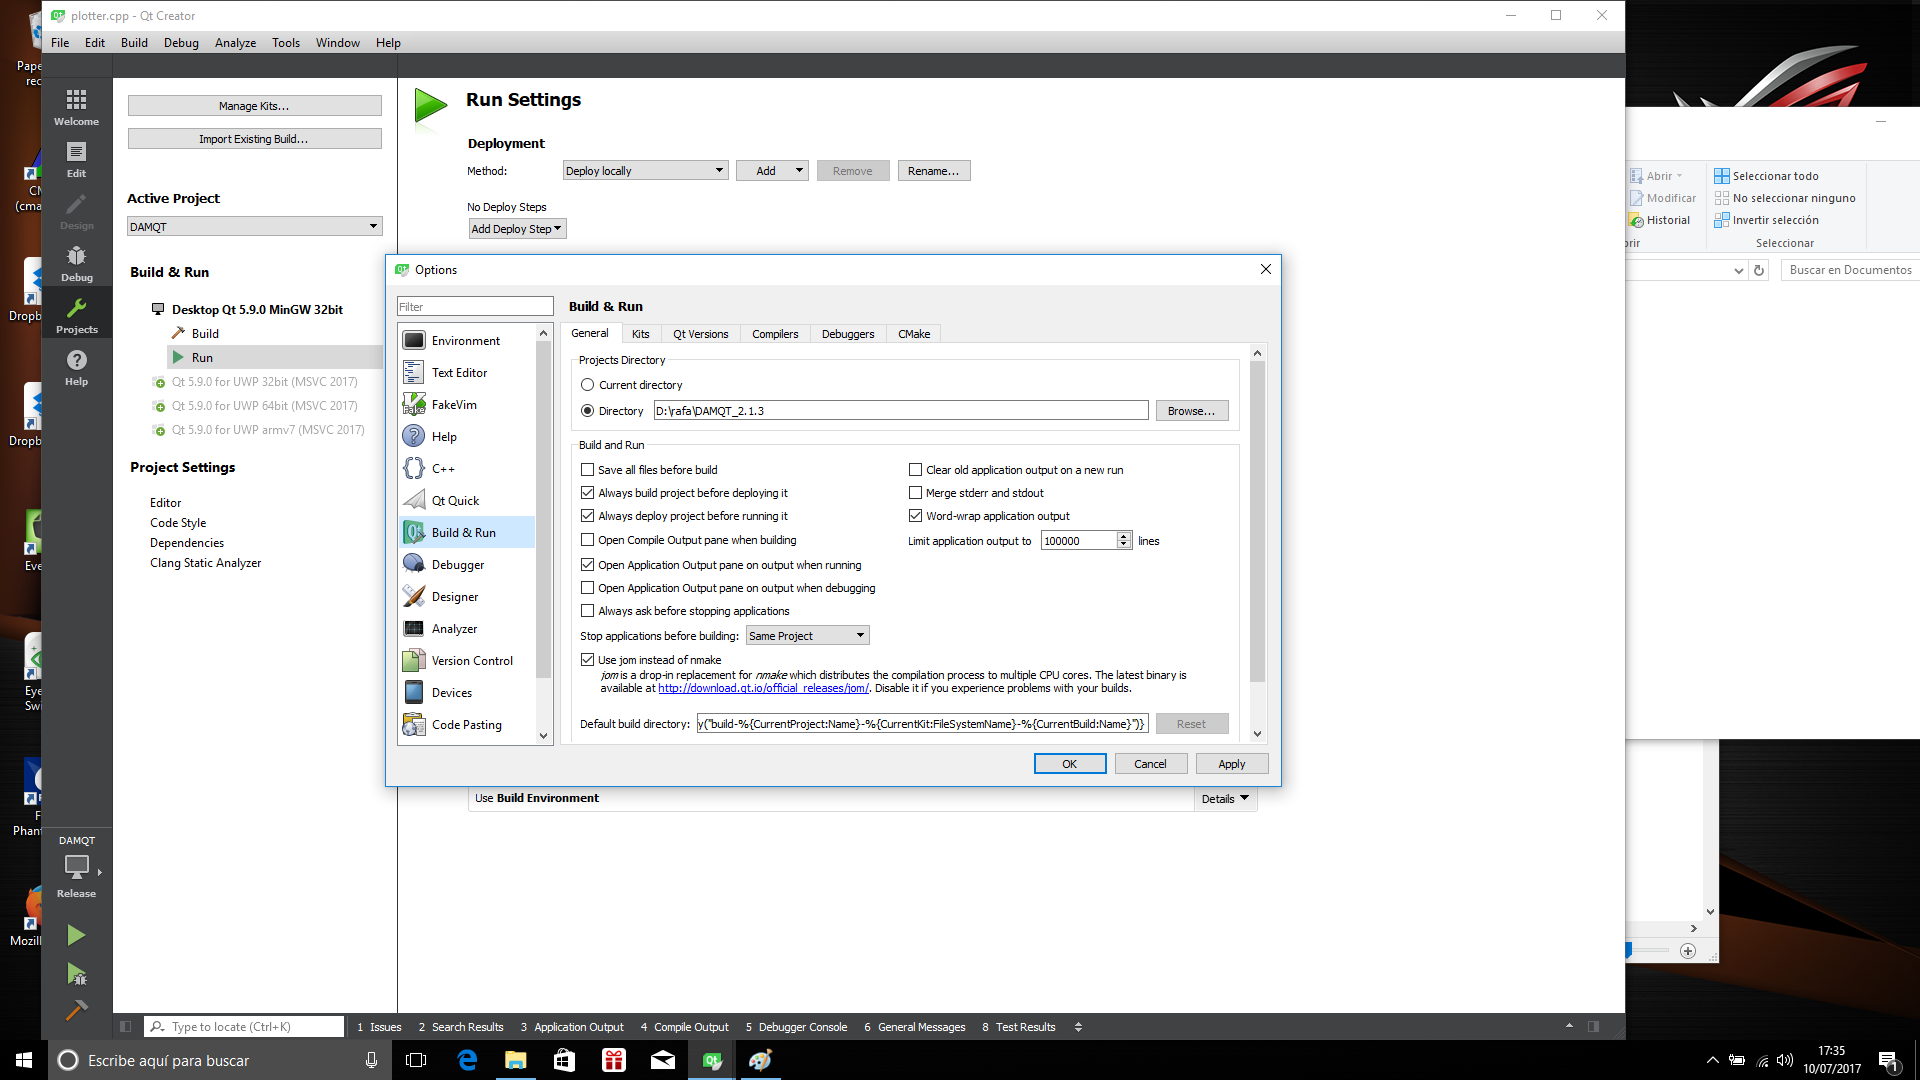
\includegraphics[width=5.5cm]{fig15.png}
\vspace*{-1mm}
\caption{\small  \label{fig:15}}
\end{center}
\end{figure}
\end{minipage}
\begin{minipage}{0.5\linewidth}
\begin{figure}[H]
\begin{center}
% \vspace*{-3mm}
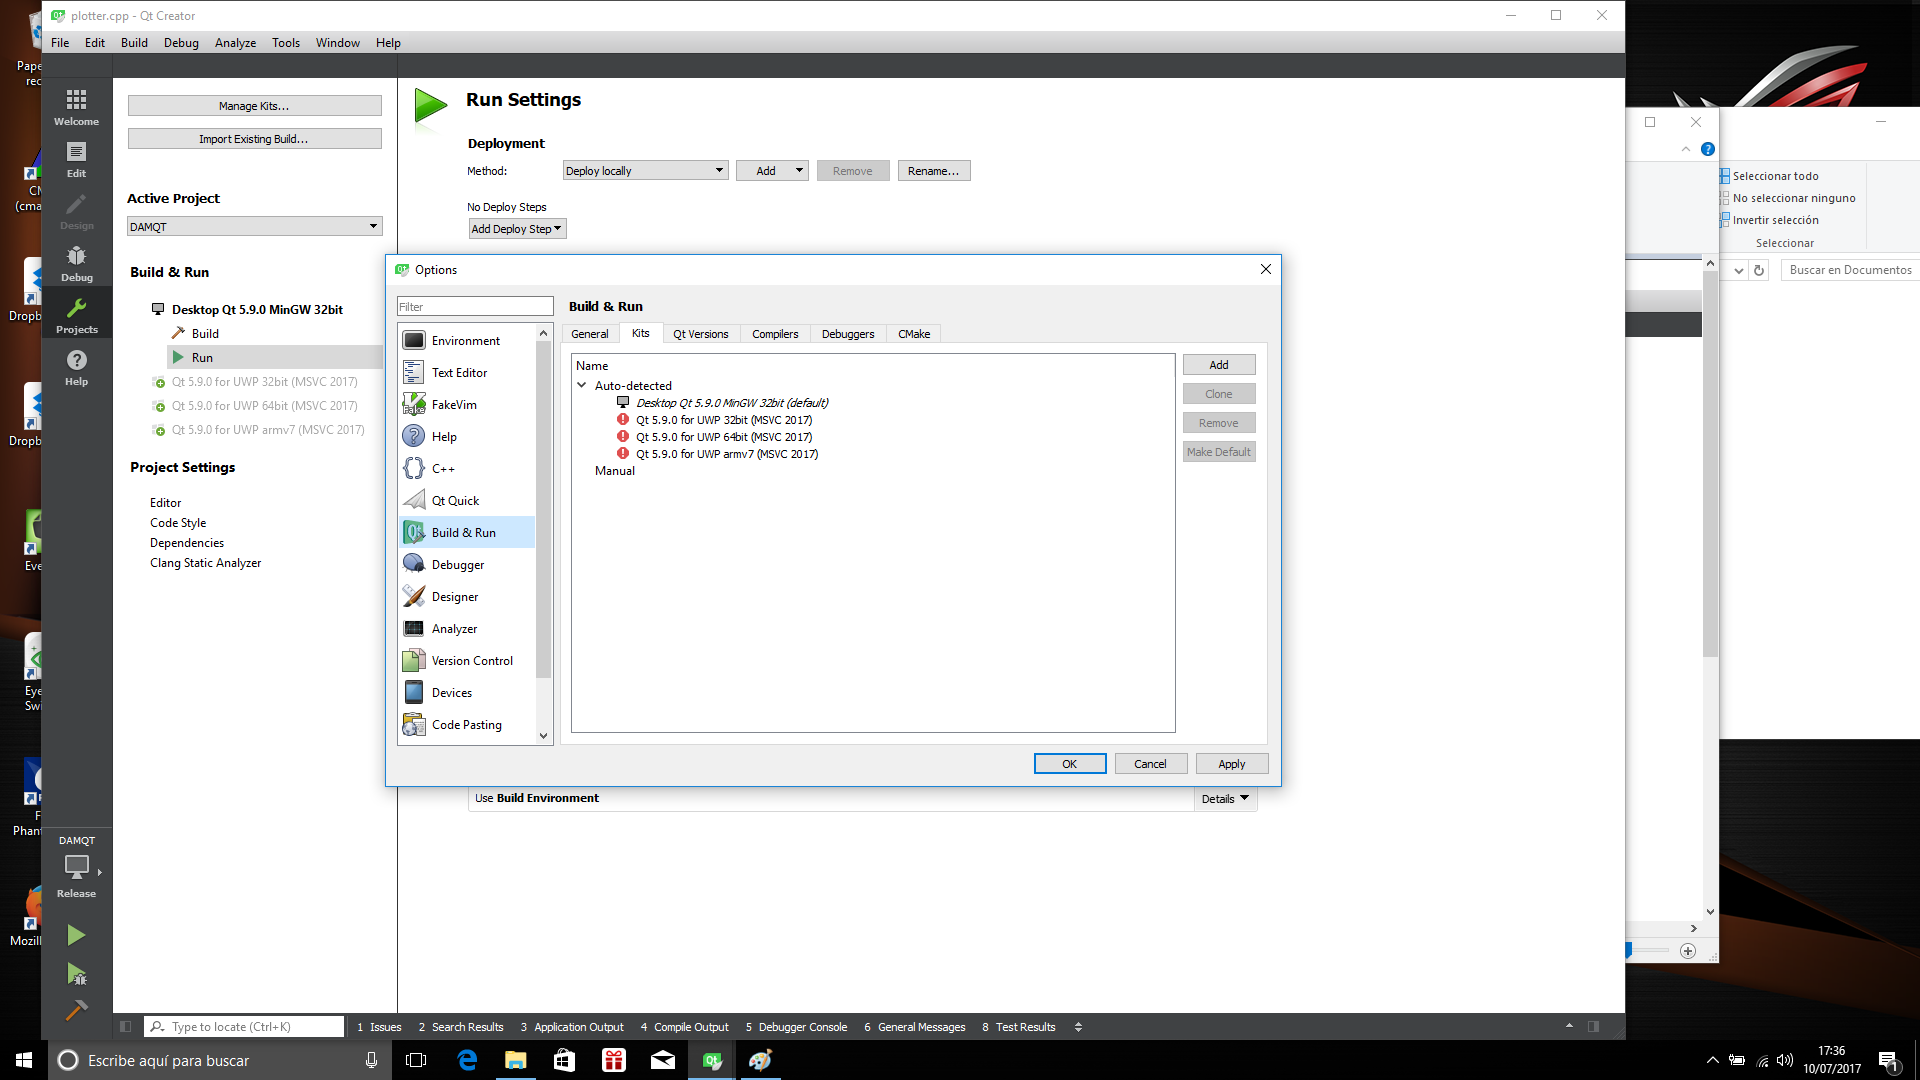
\includegraphics[width=5.5cm]{fig16.png}
\vspace*{-1mm}
\caption{\small  \label{fig:16}}
\end{center}
\end{figure}
\end{minipage}

\begin{minipage}{0.5\linewidth}
\begin{figure}[H]
\begin{center}
% \vspace*{-3mm}
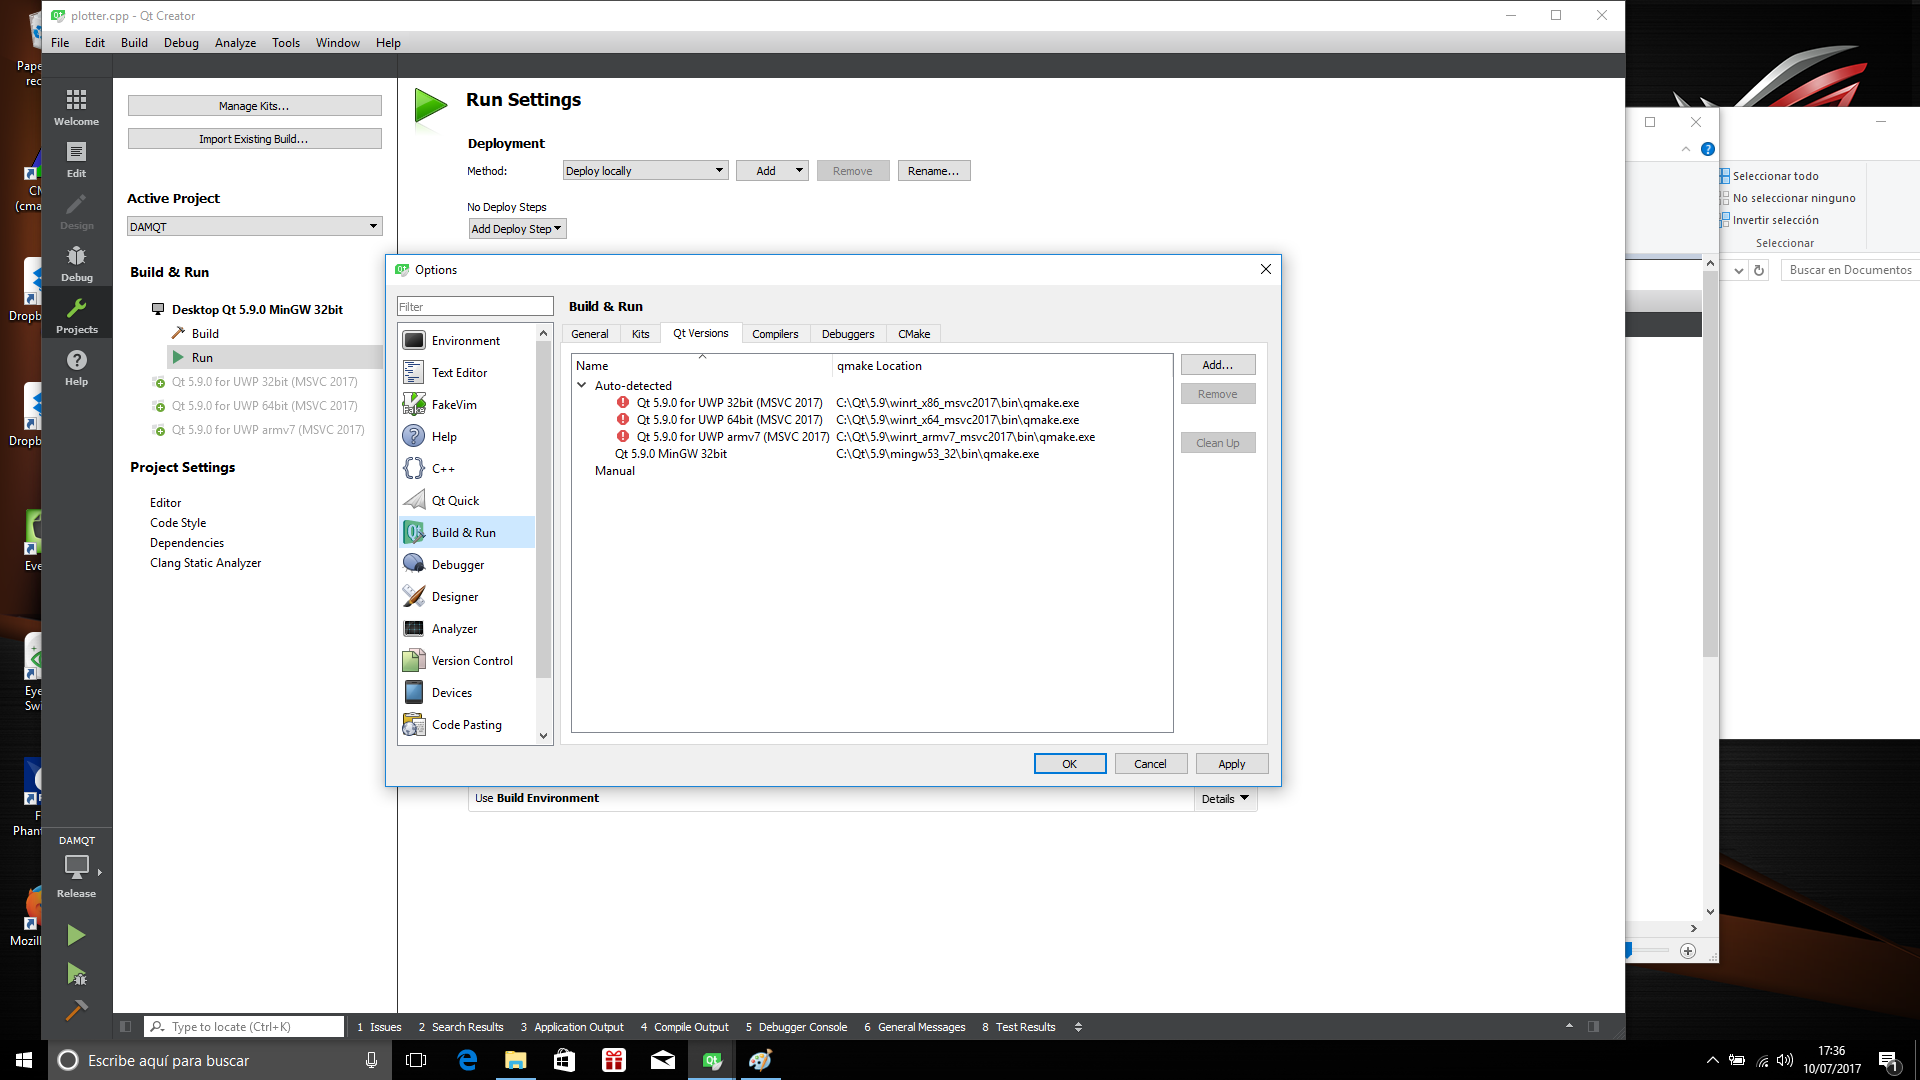
\includegraphics[width=5.5cm]{fig17.png}
\vspace*{-1mm}
\caption{\small  \label{fig:17}}
\end{center}
\end{figure}
\end{minipage}
\begin{minipage}{0.5\linewidth}
\begin{figure}[H]
\begin{center}
% \vspace*{-3mm}
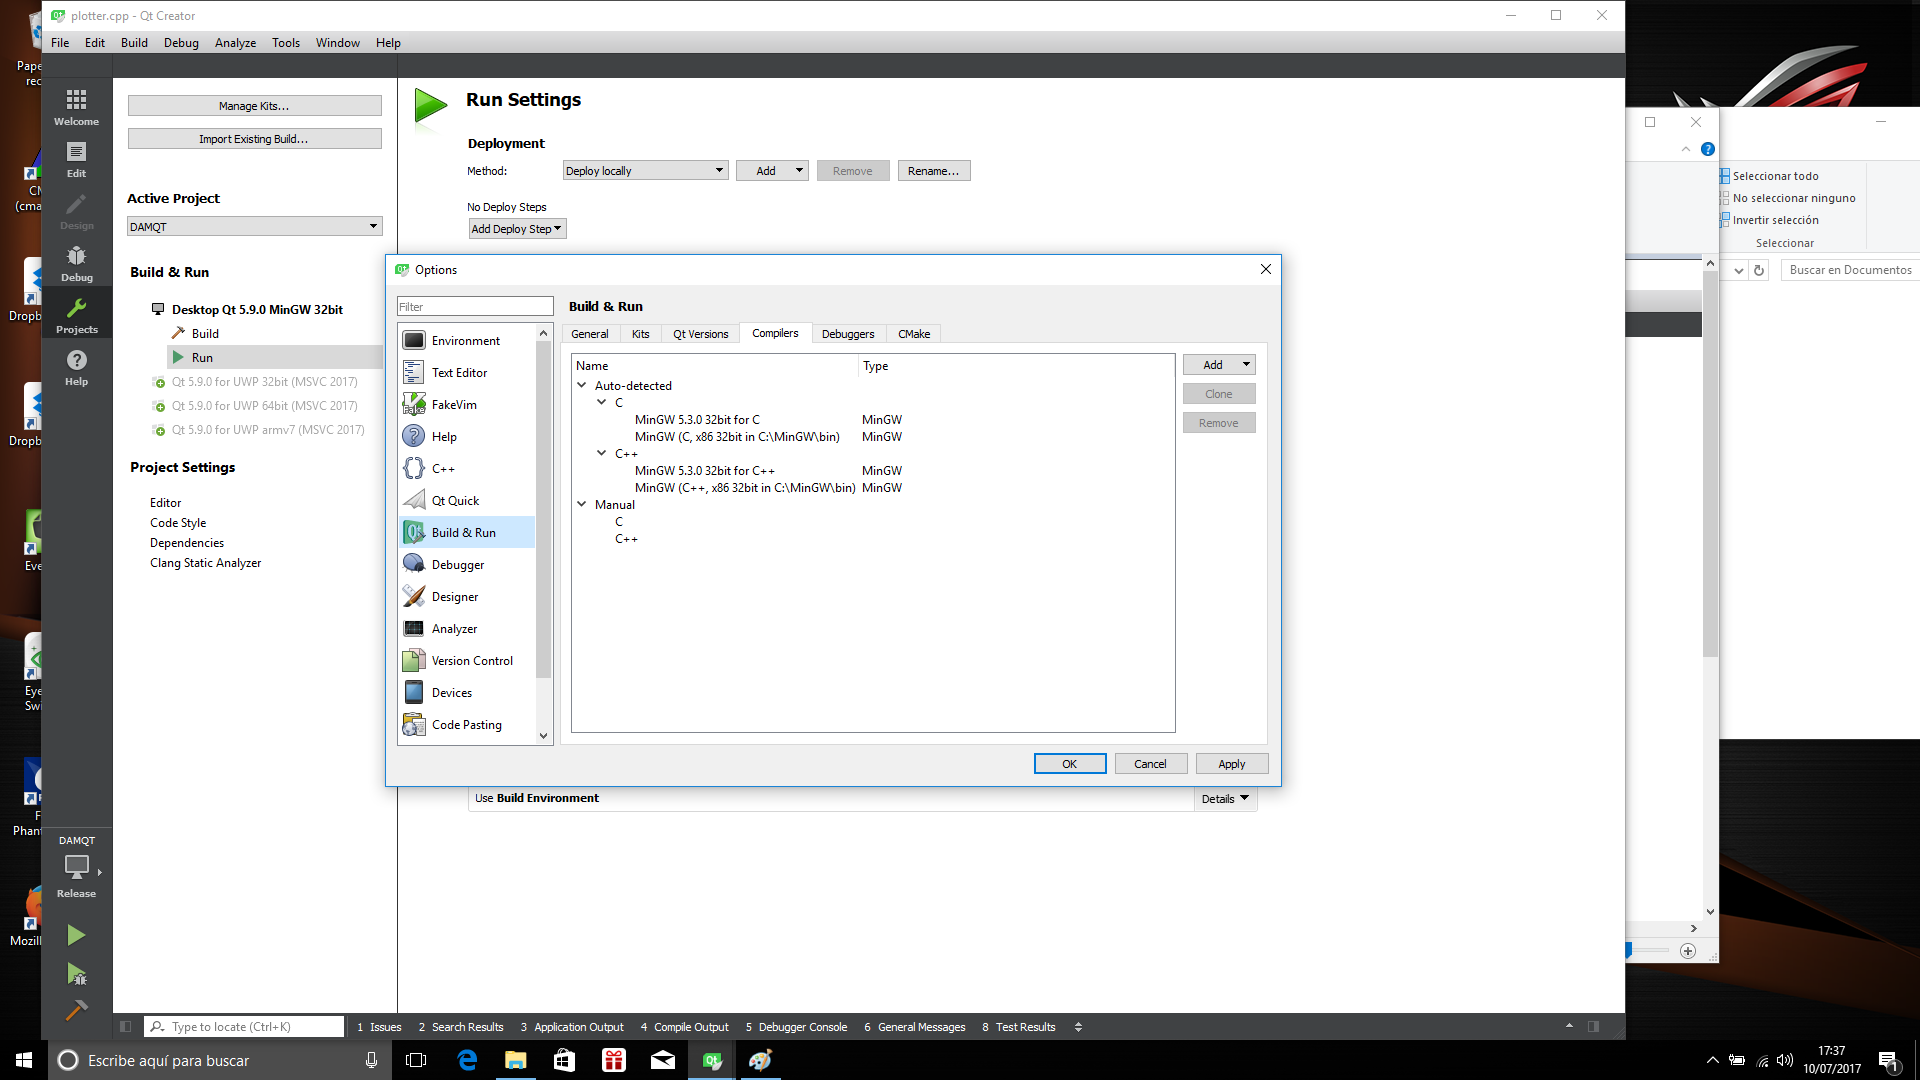
\includegraphics[width=5.5cm]{fig18.png}
\vspace*{-1mm}
\caption{\small  \label{fig:18}}
\end{center}
\end{figure}
\end{minipage}

{\it Qt versions} is also important. Again Qt 5.9.0 MinGW 32 bits must be chosen (see fig \ref{fig:17}).

{\it Compilers.} The system should detect MinGW C and C++ compilers. Otherwise, they can be added by hand
(see fig \ref{fig:18}).



{\it Debuggers.} The \texttt{gdb} debugger may be auto-detected (see fig \ref{fig:19}). This is only important if a
version of the package is to be built for debugging. In this case, the build command should be run with the option
\texttt{-DCMAKE\_BUILD\_TYPE=Debug}.

{\it CMake.} This is utmost important (see fig \ref{fig:20}). If the system does not detect \texttt{cmake}, 
it must be allocated manually.

\begin{minipage}{0.5\linewidth}
\begin{figure}[H]
\begin{center}
% \vspace*{-3mm}
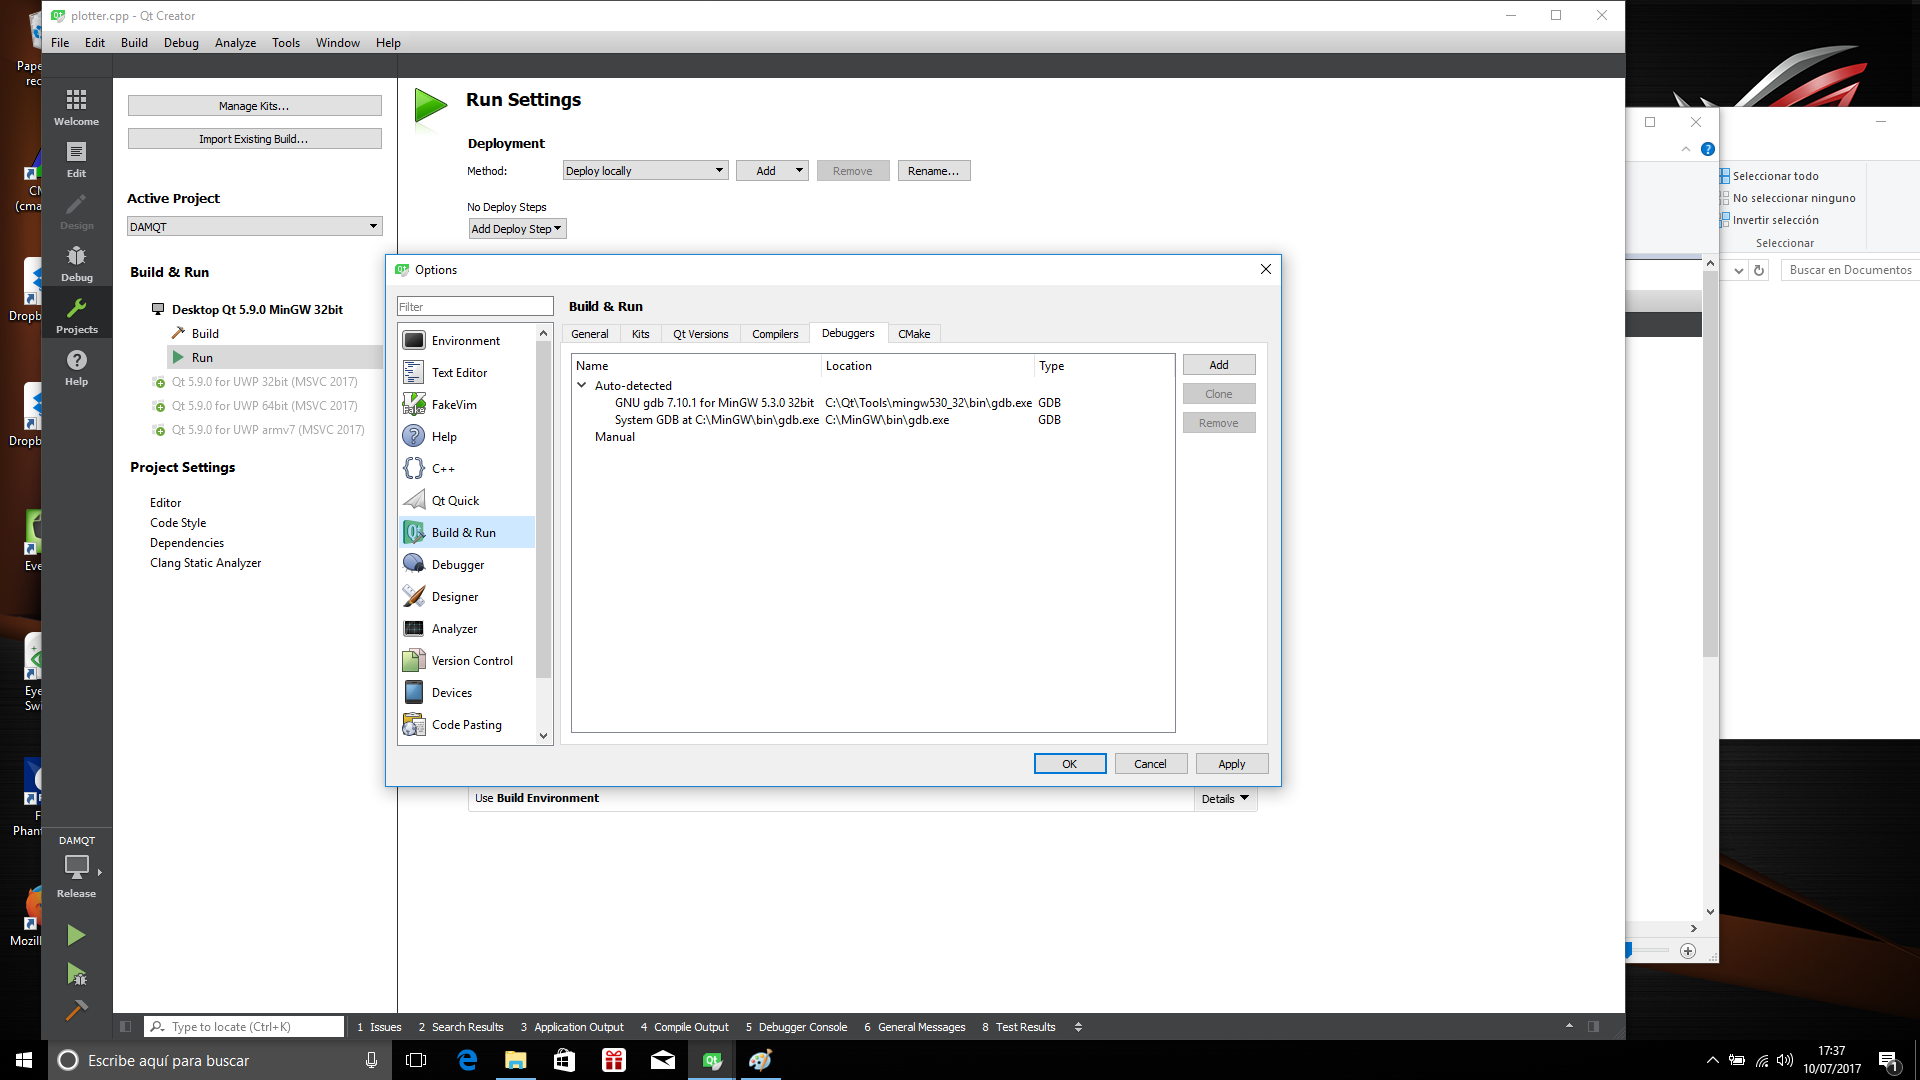
\includegraphics[width=5.5cm]{fig19.png}
\vspace*{-1mm}
\caption{\small  \label{fig:19}}
\end{center}
\end{figure}
\end{minipage}
\begin{minipage}{0.5\linewidth}
\begin{figure}[H]
\begin{center}
% \vspace*{-3mm}
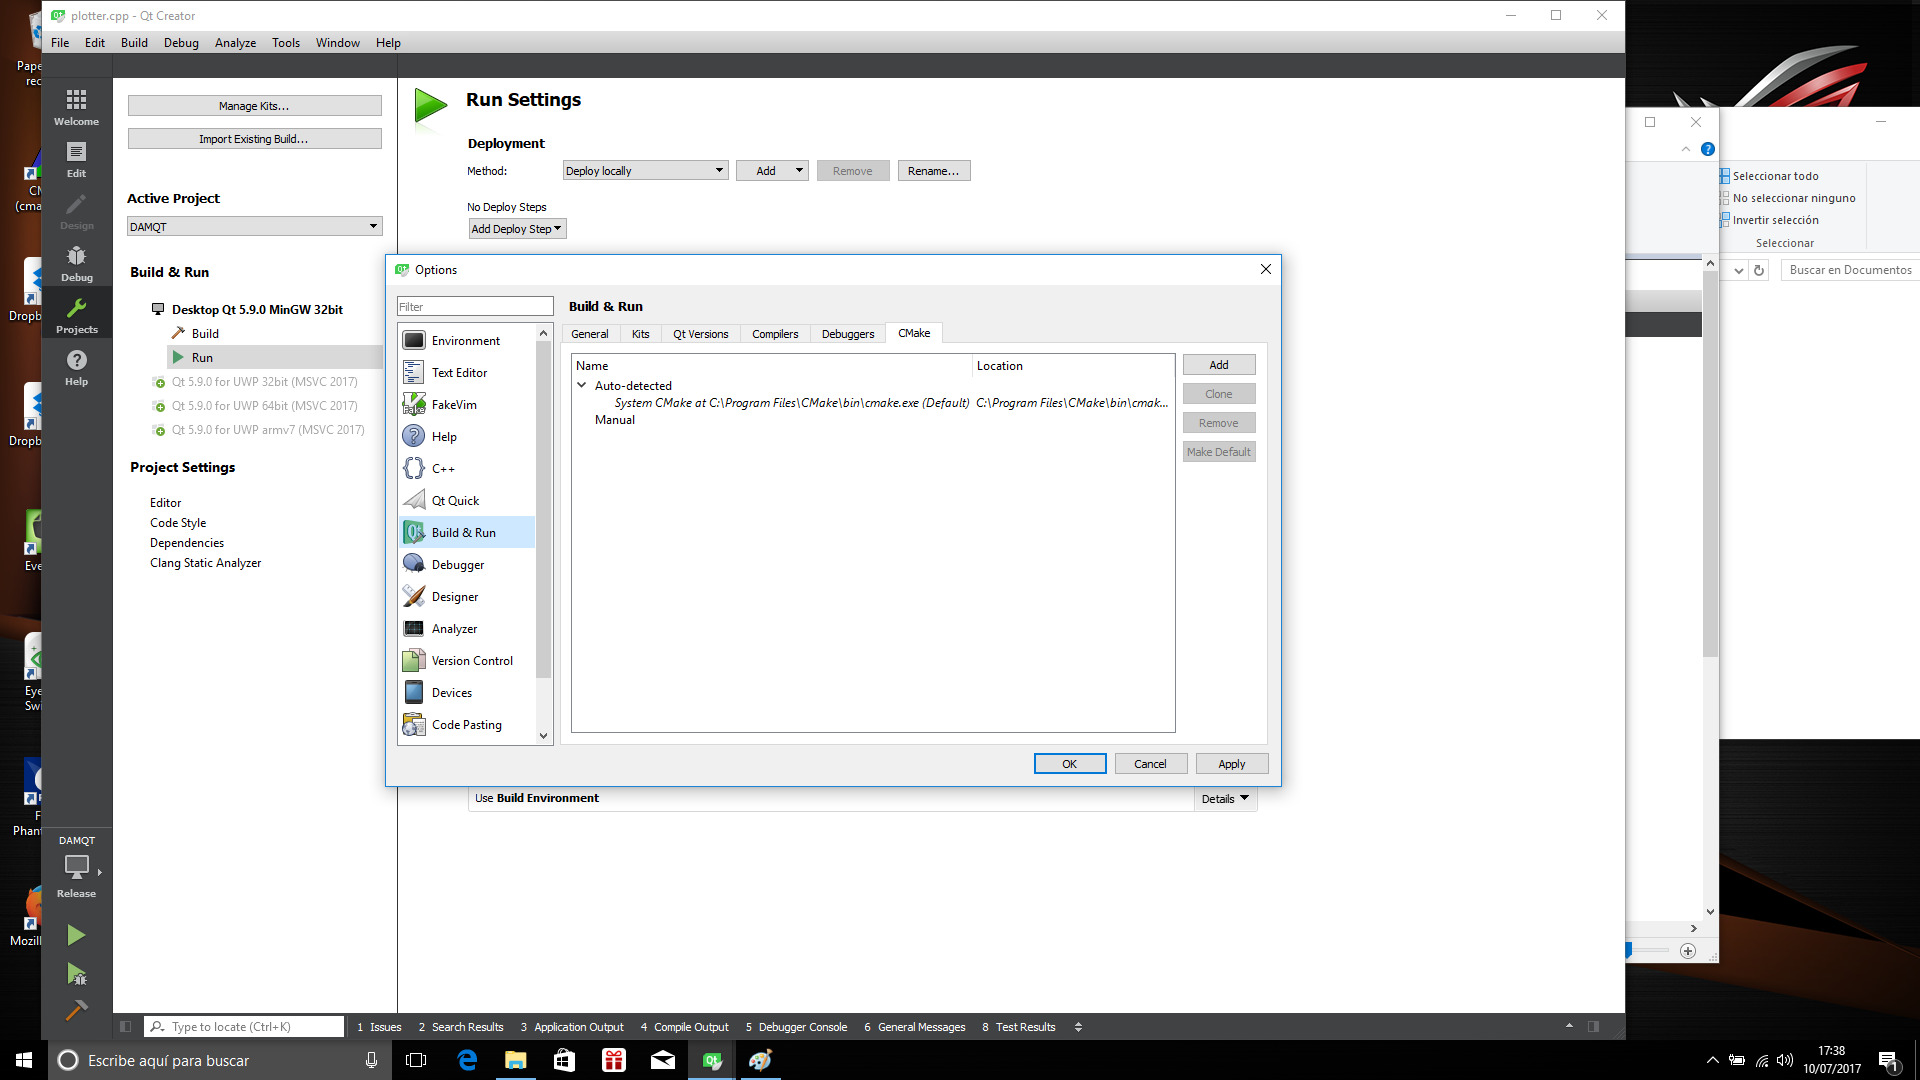
\includegraphics[width=5.5cm]{fig20.png}
\vspace*{-1mm}
\caption{\small  \label{fig:20}}
\end{center}
\end{figure}
\end{minipage}

\section{Editing files, building and running with Qt creator}

Project files can be edited by choosing the {\it Edit} option in the upper left menu of Qt creator.
This editor is particularly useful for c++ files, since it carries out dynamical checking of the code.
(See fig \ref{fig:21}).

\begin{figure}[H]
\begin{center}
% \vspace*{-3mm}
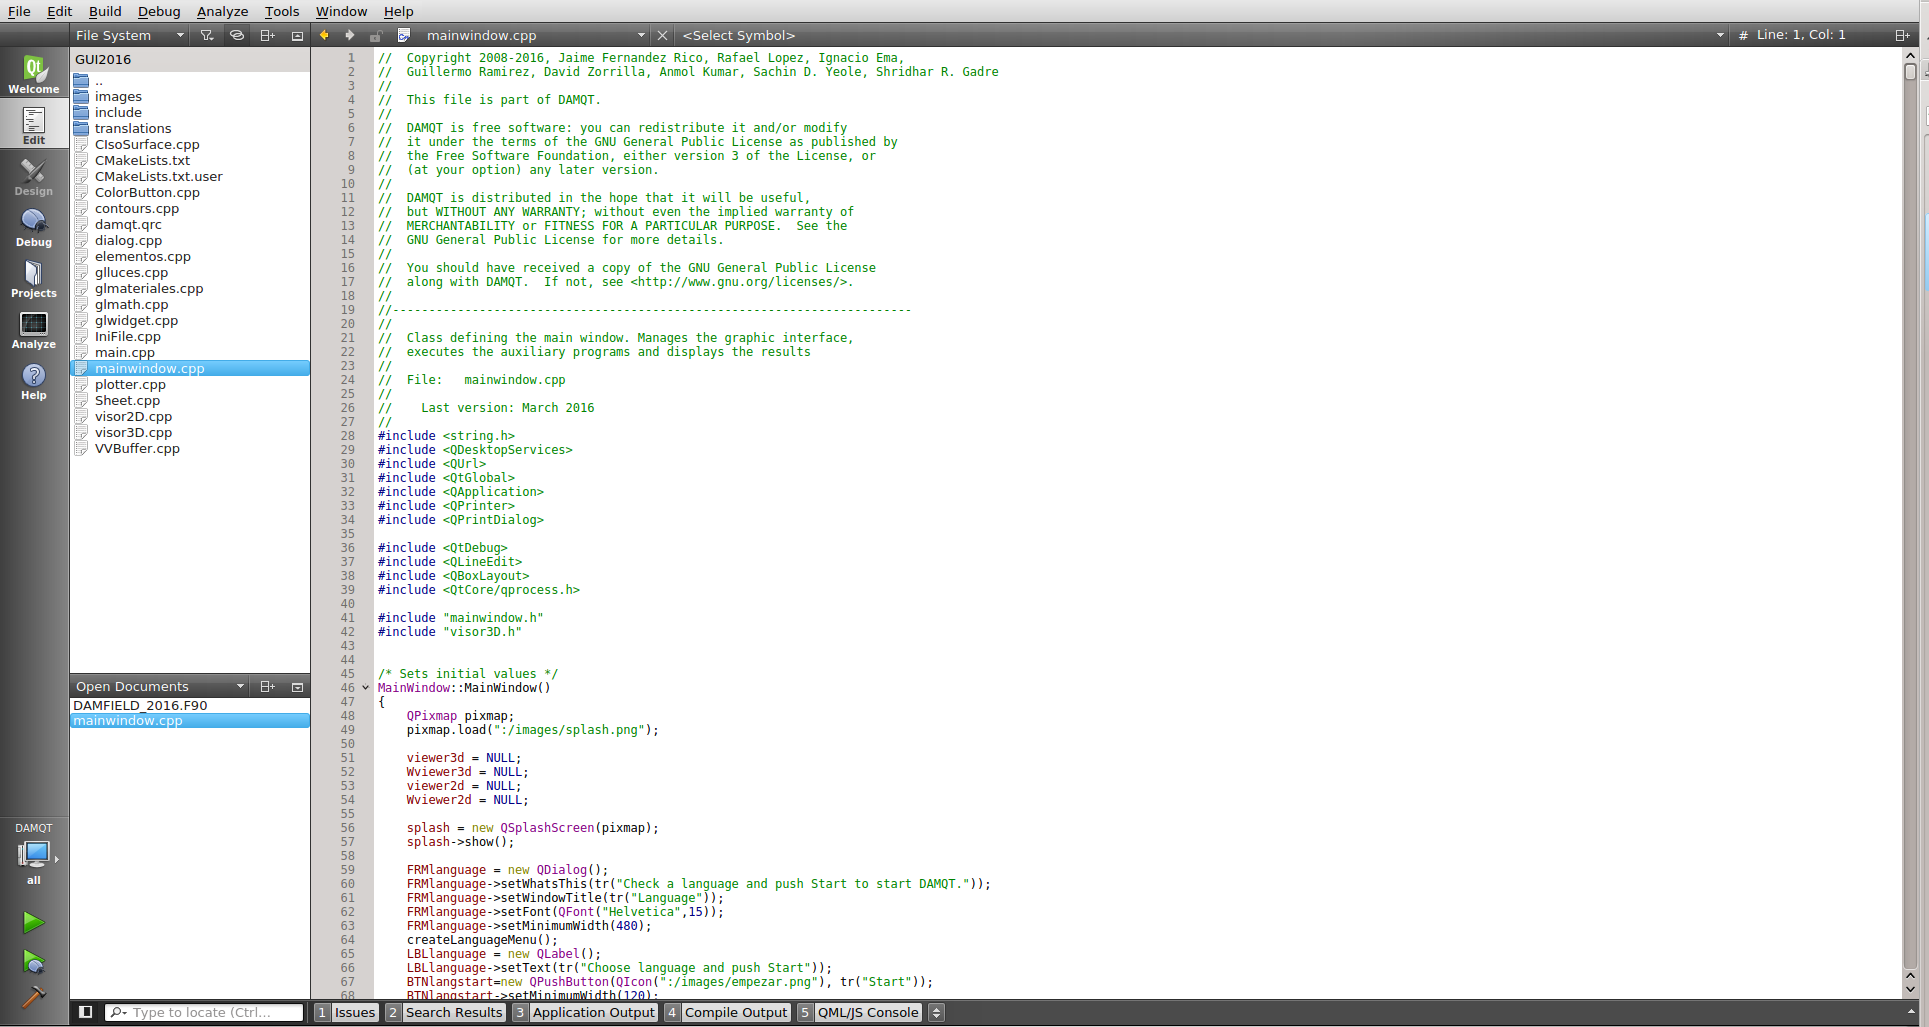
\includegraphics[width=5.5cm]{fig21.png}
\vspace*{-1mm}
\caption{\small  \label{fig:21}}
\end{center}
\end{figure}

The project can be run by pressing the green triangle in the lower left menu. If any file has
been changed since last run, it asks to save changes before building and running.

The debug mode can be launched by pressing on the green triangle with the ladybird. It only works if
the project has been built in debugging mode. Otherwise, the project will be run without debugging options.

Finally, pressing the hammer icon on the lower left menu, the project is built without running. 

A green bar shows progress in project building. The bar turns into red if severe errors are detected.
Several output screens can be displayed by choosing in the lower menu.

Once the project has been built, it is important to test that it works. This should be made before
the project is ready to create the installer. 



\section{Creating MSWindows installer with Inno Setup}

Once the project has been tested and found to work, a MSWindows installer can be prepared using Inno Setup.
The DAMQT package comes with a \texttt{.iss} file in the {\it windows} directory. This file can be loaded
into Inno Setup and modified according to the current installation.

It is not necessary to know all the subtleties of Inno Setup to make the installer. In fact, all the
required settings are present in the \texttt{.iss} file. Before running Inno Setup, it is important to check 
the suitability of the definitions of environment variables quoted in the top of the \texttt{.iss} file
(see fig \ref{fig:22}).

This suitability can be seen by looking at the \texttt{[Files]} section, where these variables are used 
as paths to the different files to be loaded in the installer. Some files refer to the executable files
in DAMQT, and other to the libraries to be loaded. Check that the quoted files exist in the
folders pointed by the pertaining variables. Otherwise, seek in your installation for the files and 
redefine the variables to point to the folders where they are contained (see fig \ref{fig:23}).

\begin{minipage}{0.5\linewidth}
\begin{figure}[H]
\begin{center}
% \vspace*{-3mm}
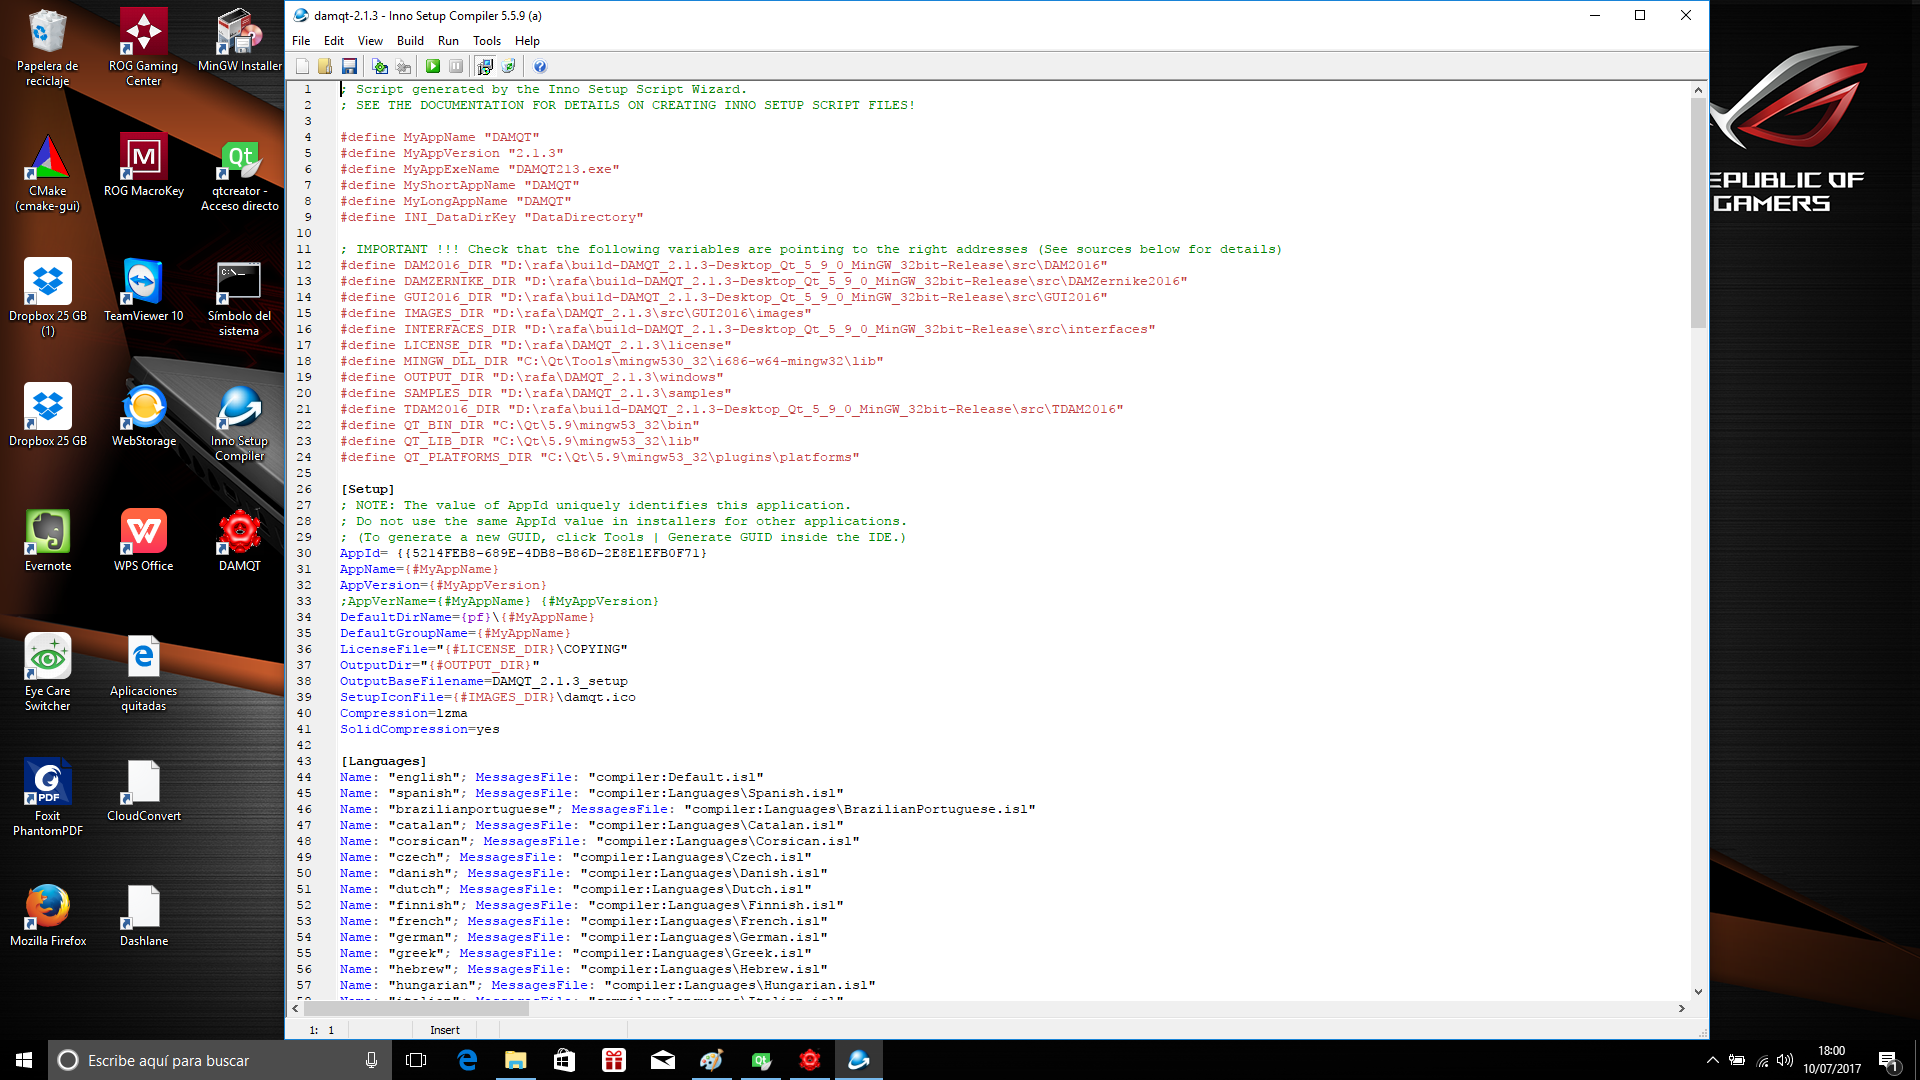
\includegraphics[width=5.5cm]{fig22.png}
\vspace*{-1mm}
\caption{\small  \label{fig:22}}
\end{center}
\end{figure}
\end{minipage}
\begin{minipage}{0.5\linewidth}
\begin{figure}[H]
\begin{center}
% \vspace*{-3mm}
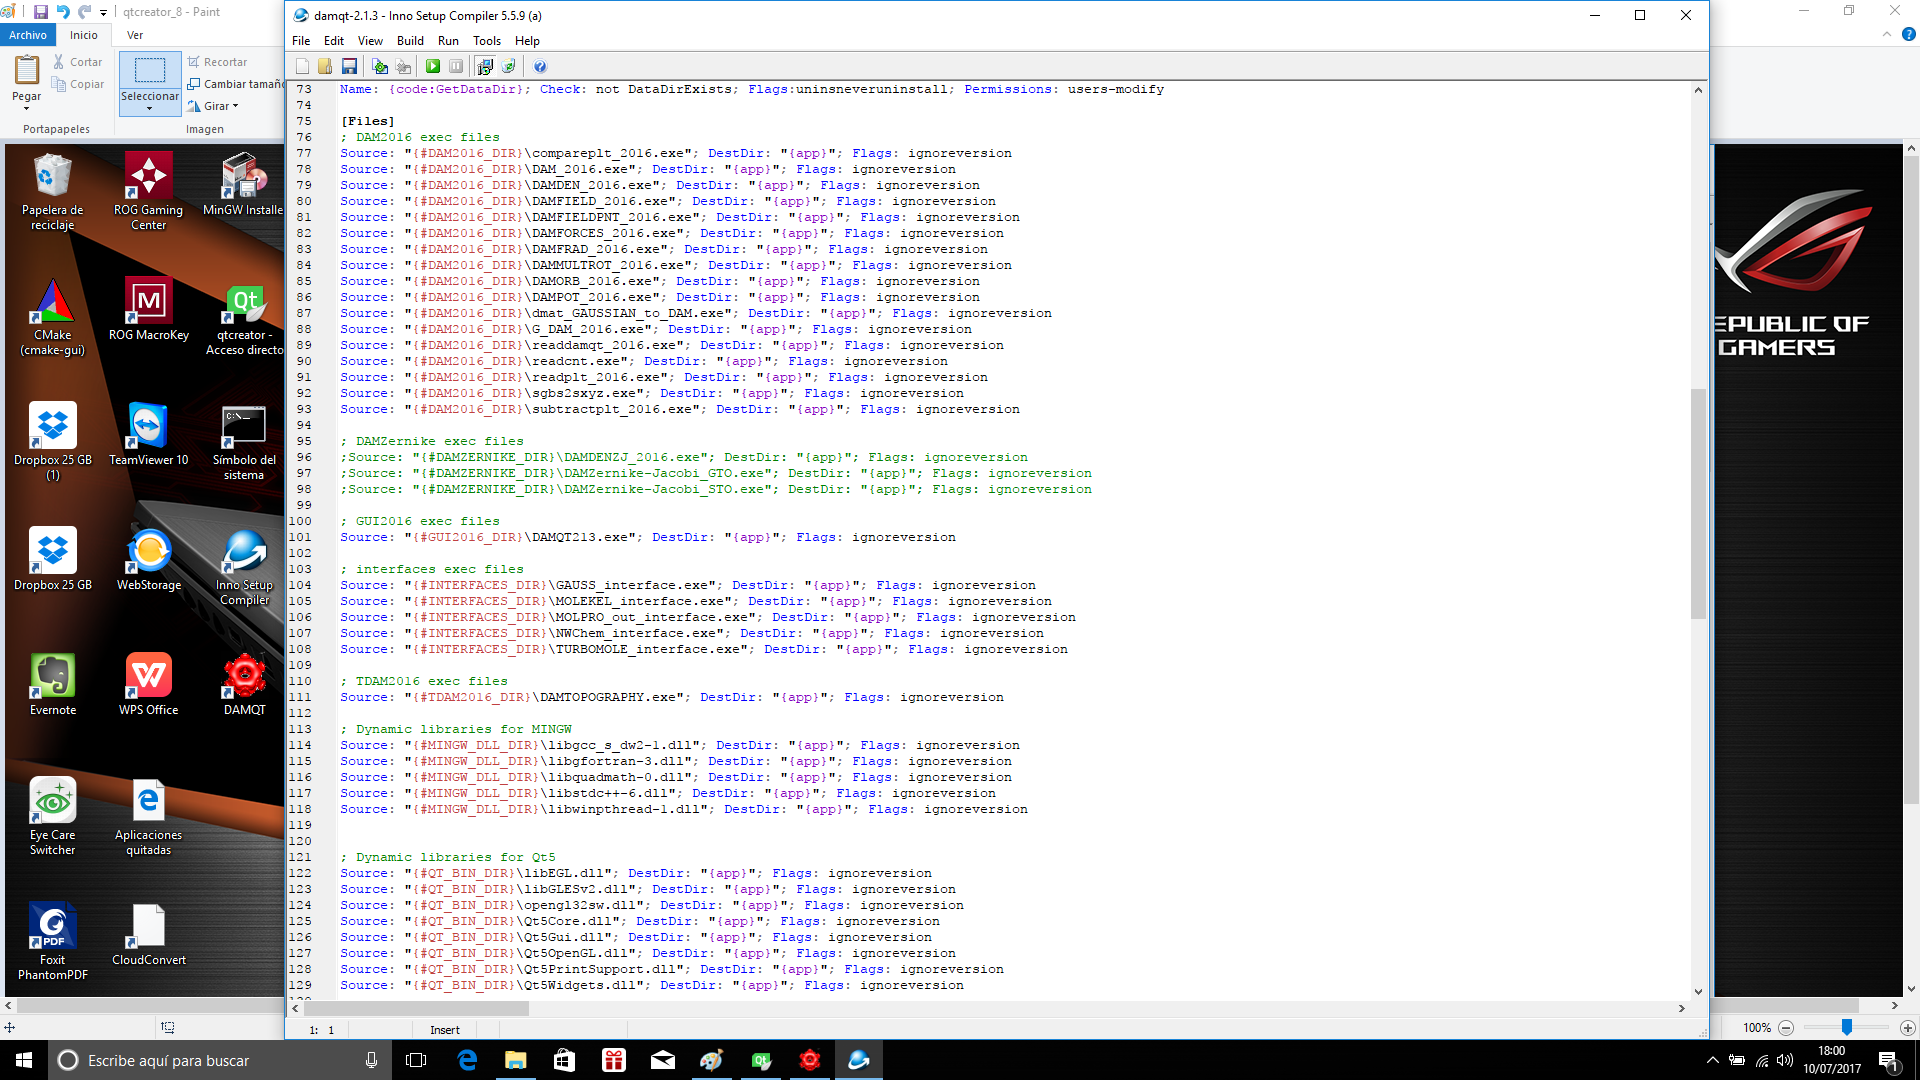
\includegraphics[width=5.5cm]{fig23.png}
\vspace*{-1mm}
\caption{\small  \label{fig:23}}
\end{center}
\end{figure}
\end{minipage}

In some cases, different libraries with the same name may appear in the installation. Choose those that
are compatible with your building choices. As a rule of thumb, libraries corresponding to MinGW are
preferable to others with equal names when available.

To generate the installer, build it with the corresponding option in Inno Setup Compiler and the run it.
You may attempt to run it directly and it will make first the building step and, if it succeeds in building, 
then will run to create the installer. This will be a file named \texttt{DAMQT\_2.1.3\_setup.exe},
ready to be run in a MSWindows environment.

The installer has been tested in windows 7, 8 and 10, and it seems to work. However, the 3D viewer fails in the
windows 7 version. 

\end{document}
